\section{Risultati}
\newcommand{\epsmx}{$\varepsilon_{max}$}
La validazione dei modelli appena discussi è stata effettuata confrontando i
risultati della simulazione con le stime dedotte dall'analisi, valutando quattro
possibili scenari contraddistinti dal valore che assume il parametro $S$.

Ognuno di questi scenari è stato simulato facendo processare al programma lo
stesso numero di job affinché le statistiche globali del sistema possano
essere confrontate. Tale numero è stato stabilito in base alle metriche che
andavano valutate ed al numero di job che le riguardava.

Lo scenario con valore di soglia $S=5$, è quello in cui soltanto circa il $2\%$
dei job di classe 2 è processato nel cloudlet e di questi circa il $90\%$
vengono interrotti, ne risulta, quindi che in relazione al numero totale dei job
che transitano nel sistema, solamente lo $0.14\%$ sono job di classe 2
processati con successo nel cloudlet e l'$1.37\%$ sono job interrotti. In
definitiva, al fine di avere una dimensione dei batch soddisfacente per il
calcolo delle relative metriche, è stato scelto un numero totale di job pari a
$500000$. In questo modo si ottiene un numero di job di classe 2 processati con
successo nel cloudlet pari a circa $700$ e un numero di job interrotti pari a
circa $6850$, ciò significa che per un valore $k=64$ corrispondente al numero
di batch, si ottengono batch di dimensione $10$ e $107$ rispettivamente, che
sono sufficienti a determinare intervalli di confidenza, seppur con un ampio
margine di errore.

Quello appena descritto è il peggior scenario possibile, in cui si registra il
minor numero di job per una determinata metrica, gli altri scenari vengono
quindi simulati tutti con un numero totale di job pari a $500000$, e a seconda
del numero di job che verranno processati nei vari nodi e della loro tipologia,
sono risultati intervalli di confidenza più o meno precisi.

Purtroppo è risultato impossibile determinare risultati attendibili per i job
di classe 1 che vengono processati nel cloud, poiché il loro numero è, per ogni
scenario, talmente esiguo, che per avere un batch di dimensione 10 sarebbero
necessari almeno 3 milioni di job in tutto. Tuttavia, con un numero di
$500000$ job totali, si ottengono delle statistiche globali molto attendibili,
infatti, ad esempio per il tempo medio di risposta del sistema, si ottiene 
una dimensione del batch pari a $\lfloor\frac{500000}{64}\rfloor = 7812$.

Per ogni statistica vengono presentati grafici e tabelle, in cui vengono
confrontati i risulatati osservati in 10 repliche della simulazione con la
relativa stima del modello analitico, inoltre nelle tabelle viene anche indicato
l'errore massimo che è stato commesso, corrispondente al massimo delle distanze 
tra la stima e l'estremo più lontano di ogni intervallo di confidenza.
%
%
%%%%%%%%%%%%%%%%%%%%%%%%%%%%%%%%%%%%%%%%%%%%%%%%%%%%%%%%%%%%%%%%%%%%%%%%%%%%%%%%
%%%%%%%%%%%%%%%%%%%%%%%%%%%%%%%%%%%%%%%%%%%%%%%%%%%%%%%%%%%%%%%%%%%%%%%%%%%%%%%%
%%%%%%%%%%%%%%%%%%%%%%%%%%%%%%%%%%%%%%%%%%%%%%%%%%%%%%%%%%%%%%%%%%%%%%%%%%%%%%%%
\subsection{Percentuale Interruzioni}
Per comprendere al meglio l'analisi delle simulazioni ed il confronto con le
stime effettuate è conveniente iniziare dalla presentazione dei risultati
riguardanti la percentuale di job di classe 2 interrotti, poiché da questi
dipendono la maggior parte delle metriche successive.

I grafici in figura~\ref{plot:intperc} mostrano che, nei casi in cui
$S=20,15,10$, la stima della percentuale di interruzione risulta leggermente
inferiore dei valori osservati nelle simulazioni e l'errore massimo che viene
commesso è di circa il $5$-$6\%$, mentre per quanto riguarda il caso in cui
$S=5$ si ottiene una stima leggermente migliore, ma ciò è dovuto al basso
valore della soglia che impedisce ai job di classe 2 di accedere al cloudlet, di
conseguenza è stata riscontrata una maggiore variabilità dei valori delle
simulazioni e si commette infatti un'errore massimo più alto pari al $7.6\%$.

La maggiore percentuale di job interrotti (circa del $30\%$ considerando le
varie repliche), si ottiene per $S=10$, mentre nei restanti due casi non si
hanno valori troppo discordanti, differiscono infatti di circa un punto
percentuale.

I valori delle simulazioni e gli errori relativi rispetto alla stima del modello
analitico sono riportati nelle
tabella~\ref{tab:intperc}.
%
\begin{figure}[!h]
\centering
%
\begin{subfigure}[t]{0.49\textwidth}
\includegraphics[width=\textwidth]{figures/simul/20_500K_intperc}
\caption{$S = 20$}
\label{20_intperc}
\end{subfigure}
%
\begin{subfigure}[t]{0.49\textwidth}
\includegraphics[width=\textwidth]{figures/simul/15_500K_intperc}
\caption{$S = 15$}
\label{15_intperc}
\end{subfigure}
%
\begin{subfigure}[t]{0.49\textwidth}
\includegraphics[width=\textwidth]{figures/simul/10_500K_intperc}
\caption{$S = 10$}
\label{10_intperc}
\end{subfigure}
%
\begin{subfigure}[t]{0.49\textwidth}
\includegraphics[width=\textwidth]{figures/simul/5_500K_intperc}
\caption{$S = 5$}
\label{5_intperc}
\end{subfigure}
%
\caption{Percentuale di interruzioni}
\label{plot:intperc}
\end{figure}
%
%
\begin{table}[!h]
\begin{adjustbox}{width=\textwidth}
\begin{tabular}{c|r@{.}l|r@{.}l|r@{.}l|r@{.}l}
& \multicolumn{2}{|c|}{$S=20$}
& \multicolumn{2}{|c}{$S=15$}
& \multicolumn{2}{|c}{$S=10$}
& \multicolumn{2}{|c}{$S=5$}
\\          
\hline
R1     & $0$&$2394 \pm 0.0003$ & $0$&$3015 \pm 0.0006$ & $0$&$2153 \pm 0.0004$ & $0$&$0217 \pm 0.0002$ \\
R2     & $0$&$2395 \pm 0.0005$ & $0$&$3004 \pm 0.0004$ & $0$&$2148 \pm 0.0005$ & $0$&$0229 \pm 0.0003$ \\
R3     & $0$&$2381 \pm 0.0003$ & $0$&$2991 \pm 0.0003$ & $0$&$2140 \pm 0.0007$ & $0$&$0204 \pm 0.0001$ \\
R4     & $0$&$2371 \pm 0.0002$ & $0$&$2996 \pm 0.0005$ & $0$&$2186 \pm 0.0013$ & $0$&$0234 \pm 0.0003$ \\
R5     & $0$&$2416 \pm 0.0005$ & $0$&$3021 \pm 0.0006$ & $0$&$2129 \pm 0.0005$ & $0$&$0227 \pm 0.0003$ \\
R6     & $0$&$2388 \pm 0.0002$ & $0$&$2983 \pm 0.0003$ & $0$&$2170 \pm 0.0008$ & $0$&$0222 \pm 0.0004$ \\
R7     & $0$&$2392 \pm 0.0008$ & $0$&$2977 \pm 0.0003$ & $0$&$2130 \pm 0.0009$ & $0$&$0217 \pm 0.0003$ \\
R8     & $0$&$2381 \pm 0.0008$ & $0$&$2991 \pm 0.0003$ & $0$&$2177 \pm 0.0005$ & $0$&$0213 \pm 0.0002$ \\
R9     & $0$&$2376 \pm 0.0003$ & $0$&$2988 \pm 0.0003$ & $0$&$2171 \pm 0.0005$ & $0$&$0233 \pm 0.0003$ \\
R10    & $0$&$2385 \pm 0.0004$ & $0$&$2997 \pm 0.0005$ & $0$&$2202 \pm 0.0010$ & $0$&$0231 \pm 0.0003$ \\
EST    & $0$&$2280$            & $0$&$2879$            & $0$&$2108$            & $0$&$0219$            \\
\epsmx & $0$&$0141 \ (5.8\%)$  & $0$&$0148 \ (4.9\%)$  & $0$&$0104 \ (4.7\%)$  & $0$&$0018 \ (7.6\%)$    
\end{tabular}
\end{adjustbox}
\caption{percentuale job di classe 2 interrotti}
\label{tab:intperc}
\end{table}

%%%%%%%%%%%%%%%%%%%%%%%%%%%%%%%%%%%%%%%%%%%%%%%%%%%%%%%%%%%%%%%%%%%%%%%%%%%%%%%%
\subsection{Tempo di Risposta Cloudlet Classe 1}
Il tempo di risposta per un job di classe 1 che viene eseguito nel cloudlet è
indipendente dal parametro S ed i risultati presentati in
figura~\ref{plot:s1clet} e nella tabella~\ref{tab:s1clet} mostrano che tutti gli
intervalli di confidenza calcolati comprendono il valore stimato ed il valore
dell'errore massimo è sotto la soglia dell'$1\%$ in ogni caso.
\begin{figure}[!h]
\centering
%
\begin{subfigure}[t]{0.49\textwidth}
\includegraphics[width=\textwidth]{figures/simul/20_500K_s1clet}
\caption{$S = 20$}
\label{20_s1clet}
\end{subfigure}
%
\begin{subfigure}[t]{0.49\textwidth}
\includegraphics[width=\textwidth]{figures/simul/15_500K_s1clet}
\caption{$S = 15$}
\label{15_s1clet}
\end{subfigure}
%
\begin{subfigure}[t]{0.49\textwidth}
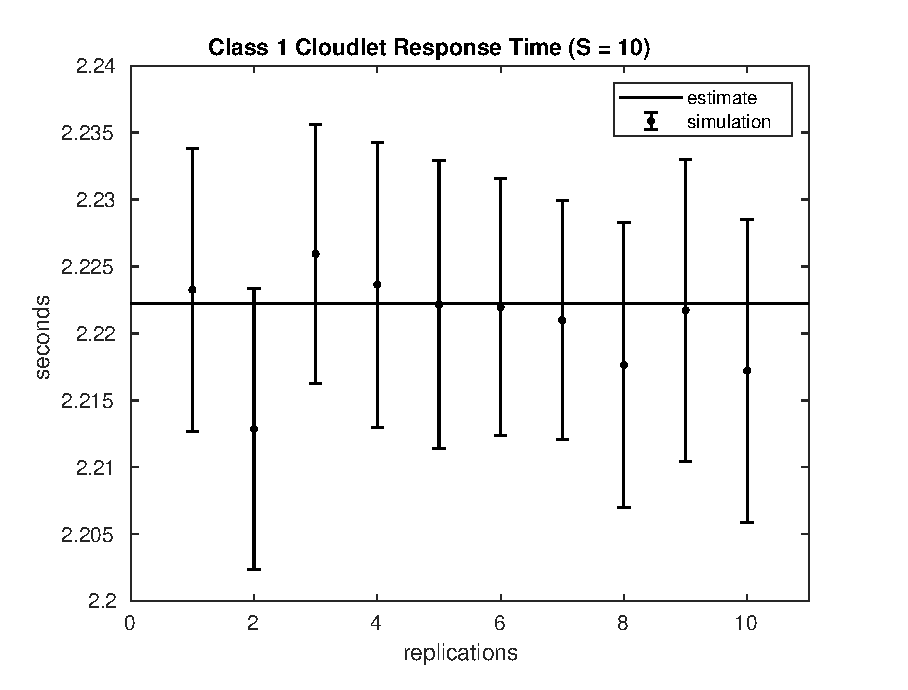
\includegraphics[width=\textwidth]{figures/simul/10_500K_s1clet}
\caption{$S = 10$}
\label{10_s1clet}
\end{subfigure}
%
\begin{subfigure}[t]{0.49\textwidth}
\includegraphics[width=\textwidth]{figures/simul/5_500K_s1clet}
\caption{$S = 5$}
\label{5_s1clet}
\end{subfigure}
%
\caption{tempo di risposta cloudlet classe 1}
\label{plot:s1clet}
\end{figure}
%
%
\begin{table}[!h]
\begin{adjustbox}{width=\textwidth}
\begin{tabular}{c|r@{.}l|r@{.}l|r@{.}l|r@{.}l}
& \multicolumn{2}{|c|}{$S=20$}
& \multicolumn{2}{|c|}{$S=15$}
& \multicolumn{2}{|c|}{$S=10$}
& \multicolumn{2}{|c}{$S=5$}
\\          
\hline
R1      & $2$&$2231 \pm 0.0105$ & $2$&$2236 \pm 0.0107$ & $2$&$2233 \pm 0.0106$ & $2$&$2231 \pm 0.0105$ \\
R2      & $2$&$2129 \pm 0.0103$ & $2$&$2131 \pm 0.0104$ & $2$&$2129 \pm 0.0105$ & $2$&$2129 \pm 0.0103$ \\
R3      & $2$&$2262 \pm 0.0096$ & $2$&$2261 \pm 0.0096$ & $2$&$2259 \pm 0.0097$ & $2$&$2262 \pm 0.0096$ \\
R4      & $2$&$2244 \pm 0.0105$ & $2$&$2165 \pm 0.0104$ & $2$&$2236 \pm 0.0106$ & $2$&$2244 \pm 0.0105$ \\
R5      & $2$&$2230 \pm 0.0107$ & $2$&$2303 \pm 0.0097$ & $2$&$2222 \pm 0.0107$ & $2$&$2230 \pm 0.0107$ \\
R6      & $2$&$2149 \pm 0.0113$ & $2$&$2218 \pm 0.0103$ & $2$&$2220 \pm 0.0096$ & $2$&$2149 \pm 0.0113$ \\
R7      & $2$&$2250 \pm 0.0106$ & $2$&$2176 \pm 0.0107$ & $2$&$2210 \pm 0.0089$ & $2$&$2250 \pm 0.0106$ \\
R8      & $2$&$2236 \pm 0.0094$ & $2$&$2171 \pm 0.0102$ & $2$&$2177 \pm 0.0107$ & $2$&$2236 \pm 0.0094$ \\
R9      & $2$&$2183 \pm 0.0104$ & $2$&$2211 \pm 0.0100$ & $2$&$2217 \pm 0.0113$ & $2$&$2183 \pm 0.0104$ \\
R10     & $2$&$2191 \pm 0.0095$ & $2$&$2168 \pm 0.0119$ & $2$&$2172 \pm 0.0113$ & $2$&$2191 \pm 0.0095$ \\
EST     & $2$&$2222$            & $2$&$2222$            & $2$&$2222$            & $2$&$2222$            \\
\epsmx  & $0$&$0136 \ (0.6\%)$  & $0$&$0178 \ (0.8\%)$  & $0$&$0134 \ (0.6\%)$  & $0$&$0136 \ (0.6\%)$    
\end{tabular}
\end{adjustbox}
\caption{tempo di risposta cloudlet classe 1}
\label{tab:s1clet}
\end{table}

%%%%%%%%%%%%%%%%%%%%%%%%%%%%%%%%%%%%%%%%%%%%%%%%%%%%%%%%%%%%%%%%%%%%%%%%%%%%%%%%
\subsection{Tempo di Risposta Cloudlet Classe 2}
La figura~\ref{plot:s2clet} e la tabella~\ref{tab:s2clet} mostrano un tempo di
risposta medio per i job di classe 2 eseguiti nel cloudlet che cresce/decresce
in modo proporzionale ad $S$, ciò sta a indicare che la probabilità di
interruzione di un job in esecuzione nel cloudlet ($P_{intr}^{clet}$) è
inversamente proporzionale a $S$ ed incide maggiormente nell'abbattimento del
tempo di risposta laddove $S$ è minore.

La stima effettuata, nei casi in cui $S=20,15,10$, è affidabile con un errore
massimo del $5\%$, mentre, nel caso in cui $S=5$, gli intervalli di confidenza
hanno un ampiezza eccessiva con un errore anche del $104\%$, quest'ultimo fatto
è dovuto al basso valore del parametro di soglia e all'elevato tasso di
interruzione per i job accettati nel nodo, risulta così un ridotto numero di job
di classe 2 che vengono processati nel cloudlet, e di conseguenza una dimensione
dei batch troppo piccola per ottenere intervalli precisi.
\begin{figure}[!h]
\centering
%
\begin{subfigure}[t]{0.49\textwidth}
\includegraphics[width=\textwidth]{figures/simul/20_500K_s2clet}
\caption{$S = 20$}
\label{20_s2clet}
\end{subfigure}
%
\begin{subfigure}[t]{0.49\textwidth}
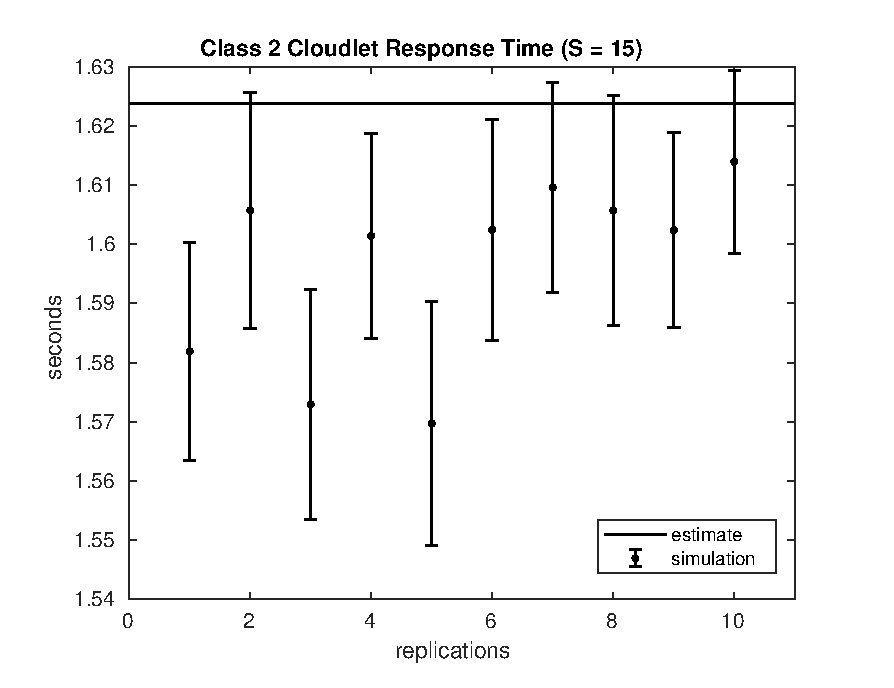
\includegraphics[width=\textwidth]{figures/simul/15_500K_s2clet}
\caption{$S = 15$}
\label{15_s2clet}
\end{subfigure}
%
\begin{subfigure}[t]{0.49\textwidth}
\includegraphics[width=\textwidth]{figures/simul/10_500K_s2clet}
\caption{$S = 10$}
\label{10_s2clet}
\end{subfigure}
%
\begin{subfigure}[t]{0.49\textwidth}
\includegraphics[width=\textwidth]{figures/simul/5_500K_s2clet}
\caption{$S = 5$}
\label{5_s2clet}
\end{subfigure}
%
\caption{tempo di risposta cloudlet classe 2}
\label{plot:s2clet}
\end{figure}
%
%
\begin{table}[!h]
\begin{adjustbox}{width=\textwidth}
\begin{tabular}{c|r@{.}l|r@{.}l|r@{.}l|r@{.}l}
& \multicolumn{2}{|c|}{$S=20$}
& \multicolumn{2}{|c|}{$S=15$}
& \multicolumn{2}{|c|}{$S=10$}
& \multicolumn{2}{|c}{$S=5$}
\\          
\hline
R1      & $2$&$4074 \pm 0.0153$ & $1$&$5819 \pm 0.0184$ & $0$&$8151 \pm 0.0187$ & $0$&$4265 \pm 0.0976$  \\
R2      & $2$&$4115 \pm 0.0172$ & $1$&$6057 \pm 0.0200$ & $0$&$8441 \pm 0.0228$ & $0$&$3558 \pm 0.0302$  \\
R3      & $2$&$3949 \pm 0.0164$ & $1$&$5730 \pm 0.0195$ & $0$&$7968 \pm 0.0199$ & $0$&$4156 \pm 0.1189$  \\
R4      & $2$&$4221 \pm 0.0175$ & $1$&$6014 \pm 0.0173$ & $0$&$8314 \pm 0.0185$ & $0$&$5185 \pm 0.3093$  \\
R5      & $2$&$4125 \pm 0.0172$ & $1$&$5697 \pm 0.0206$ & $0$&$8237 \pm 0.0203$ & $0$&$4449 \pm 0.2161$  \\
R6      & $2$&$3891 \pm 0.0148$ & $1$&$6024 \pm 0.0186$ & $0$&$8139 \pm 0.0196$ & $0$&$4307 \pm 0.1697$  \\
R7      & $2$&$3929 \pm 0.0173$ & $1$&$6096 \pm 0.0178$ & $0$&$8136 \pm 0.0173$ & $0$&$4085 \pm 0.1162$  \\
R8      & $2$&$3962 \pm 0.0168$ & $1$&$6057 \pm 0.0194$ & $0$&$8197 \pm 0.0186$ & $0$&$4874 \pm 0.3175$  \\
R9      & $2$&$4046 \pm 0.0167$ & $1$&$6024 \pm 0.0165$ & $0$&$8232 \pm 0.0241$ & $0$&$4984 \pm 0.2696$  \\
R10     & $2$&$4107 \pm 0.0168$ & $1$&$6139 \pm 0.0155$ & $0$&$8296 \pm 0.0242$ & $0$&$5865 \pm 0.4225$  \\
EST     & $2$&$3904$            & $1$&$6238$            & $0$&$8425$            & $0$&$3980$             \\
\epsmx  & $0$&$0492 \ (2.0\%)$  & $0$&$0336 \ (2.1\%)$  & $0$&$0258 \ (3.2\%)$  & $0$&$6110 \ (104.2\%)$   
\end{tabular}
\end{adjustbox}
\caption{tempo di risposta cloudlet classe 2}
\label{tab:s2clet}
\end{table}

%%%%%%%%%%%%%%%%%%%%%%%%%%%%%%%%%%%%%%%%%%%%%%%%%%%%%%%%%%%%%%%%%%%%%%%%%%%%%%%%%
\subsection{Tempo di Risposta Cloudlet}
I risultati della simulazione (figura~\ref{plot:sclet} e
tabella~\ref{tab:sclet}) mostrano come il clodlet reagisce in base ai diversi
scenari:
\begin{itemize}
\item[$S=5$ :] l'esiguo numero di job di classe 2 processati nel cloudlet
discusso in precedenza, fa sì che nel cloudlet è come se fossero eseguiti
soltanto job di classe 1, infatti il tempo di risposta medio globale del nodo è
molto vicino al tempo di risposta medio di quest'ultimi;
\item[$S=20$ :] in questo caso le interruzioni comportano una riduzione
significativa del tempo di servizio medio dei job di classe 2, pertanto il tempo
di risposta medio globale del cloudlet ne risulta attenuato;
\item[$S=10,15$ :] il maggior numero di interruzioni riduce di molto il tempo di
servizio medio dei job di classe 2, in maniera tale da portare il tempo di
risposta medio globale del cloudlet al di sotto del tempo che si avrebbe nel
caso in cui fossero eseguiti soltanto job di classe 1.
\end{itemize}

Le stime effettuate si avvicinano ai valori delle simulazioni con un errore che
va dallo $0.7\%$ del caso in cui $S=10$ all' $1.7\%$ del caso in cui $S=5$.
Degno di nota è il fatto che, in quest'ultimo caso, l'errore sulla stima della
statistica di classe 2 precedente, non abbia inciso particolarmente, sempre
per via dell'esiguo numero di job processati della suddetta classe.
\begin{figure}[!h]
\centering
%
\begin{subfigure}[t]{0.49\textwidth}
\includegraphics[width=\textwidth]{figures/simul/20_500K_sclet}
\caption{$S = 20$}
\label{20_sclet}
\end{subfigure}
%
\begin{subfigure}[t]{0.49\textwidth}
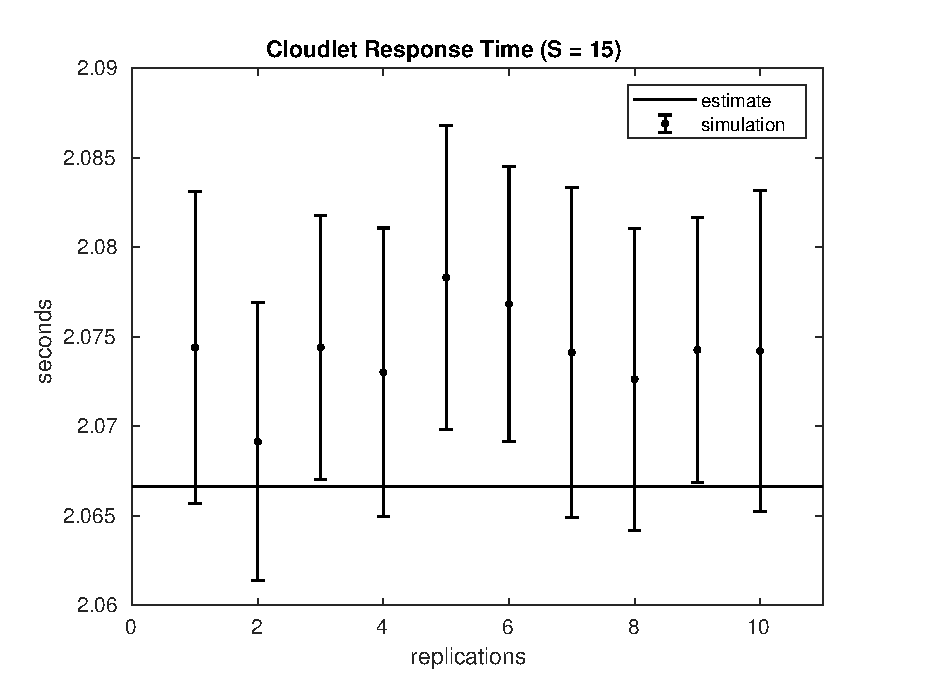
\includegraphics[width=\textwidth]{figures/simul/15_500K_sclet}
\caption{$S = 15$}
\label{15_sclet}
\end{subfigure}
%
\begin{subfigure}[t]{0.49\textwidth}
\includegraphics[width=\textwidth]{figures/simul/10_500K_sclet}
\caption{$S = 10$}
\label{10_sclet}
\end{subfigure}
%
\begin{subfigure}[t]{0.49\textwidth}
\includegraphics[width=\textwidth]{figures/simul/5_500K_sclet}
\caption{$S = 5$}
\label{5_sclet}
\end{subfigure}
%
\caption{tempo di risposta cloudlet}
\label{plot:sclet}
\end{figure}
%
%
\begin{table}[!h]
\begin{adjustbox}{width=\textwidth}
\begin{tabular}{c|r@{.}l|r@{.}l|r@{.}l|r@{.}l}
& \multicolumn{2}{|c|}{$S=20$}
& \multicolumn{2}{|c|}{$S=15$}
& \multicolumn{2}{|c|}{$S=10$}
& \multicolumn{2}{|c}{$S=5$}
\\          
\hline
R1      & $2$&$2922 \pm 0.0067$ & $2$&$0744 \pm 0.0087$ & $2$&$1240 \pm 0.0115$ & $2$&$2171 \pm 0.0107$ \\
R2      & $2$&$2885 \pm 0.0082$ & $2$&$0691 \pm 0.0078$ & $2$&$1123 \pm 0.0115$ & $2$&$2070 \pm 0.0109$ \\
R3      & $2$&$2896 \pm 0.0081$ & $2$&$0744 \pm 0.0074$ & $2$&$1265 \pm 0.0104$ & $2$&$2207 \pm 0.0102$ \\
R4      & $2$&$2996 \pm 0.0073$ & $2$&$0730 \pm 0.0081$ & $2$&$1213 \pm 0.0114$ & $2$&$2186 \pm 0.0113$ \\
R5      & $2$&$2942 \pm 0.0072$ & $2$&$0783 \pm 0.0085$ & $2$&$1221 \pm 0.0110$ & $2$&$2165 \pm 0.0099$ \\
R6      & $2$&$2811 \pm 0.0079$ & $2$&$0768 \pm 0.0077$ & $2$&$1204 \pm 0.0102$ & $2$&$2160 \pm 0.0108$ \\
R7      & $2$&$2885 \pm 0.0074$ & $2$&$0741 \pm 0.0092$ & $2$&$1216 \pm 0.0103$ & $2$&$2147 \pm 0.0094$ \\
R8      & $2$&$2885 \pm 0.0071$ & $2$&$0726 \pm 0.0084$ & $2$&$1151 \pm 0.0112$ & $2$&$2185 \pm 0.0098$ \\
R9      & $2$&$2887 \pm 0.0079$ & $2$&$0743 \pm 0.0074$ & $2$&$1191 \pm 0.0115$ & $2$&$2150 \pm 0.0110$ \\
R10     & $2$&$2918 \pm 0.0066$ & $2$&$0742 \pm 0.0090$ & $2$&$1141 \pm 0.0127$ & $2$&$2101 \pm 0.0106$ \\
EST     & $2$&$2884$            & $2$&$0666$            & $2$&$1002$            & $2$&$2147$            \\
\epsmx  & $0$&$0185 \ (0.8\%)$  & $0$&$0201 \ (1.0\%)$  & $0$&$0367 \ (1.7\%)$  & $0$&$0162 \ (0.7\%)$    
\end{tabular}
\end{adjustbox}
\caption{tempo di risposta cloudlet}
\label{tab:sclet}
\end{table}

%%%%%%%%%%%%%%%%%%%%%%%%%%%%%%%%%%%%%%%%%%%%%%%%%%%%%%%%%%%%%%%%%%%%%%%%%%%%%%%%
\subsection{Tempo di Risposta Cloud Classe 2}
Il tempo di risposta per un job di classe 2 che viene eseguito nel cloud è
indipendente dal parametro S ed i risultati presentati in
figura~\ref{plot:s2cloud} e nella tabella~\ref{tab:s2cloud} mostrano che tutti
gli intervalli di confidenza calcolati comprendono il valore stimato ed il
valore dell'errore massimo è sotto la soglia dell'$1\%$ in ogni caso.
\begin{figure}[!h]
\centering
%
\begin{subfigure}[t]{0.49\textwidth}
\includegraphics[width=\textwidth]{figures/simul/20_500K_s2cloud}
\caption{$S = 20$}
\label{20_s2cloud}
\end{subfigure}
%
\begin{subfigure}[t]{0.49\textwidth}
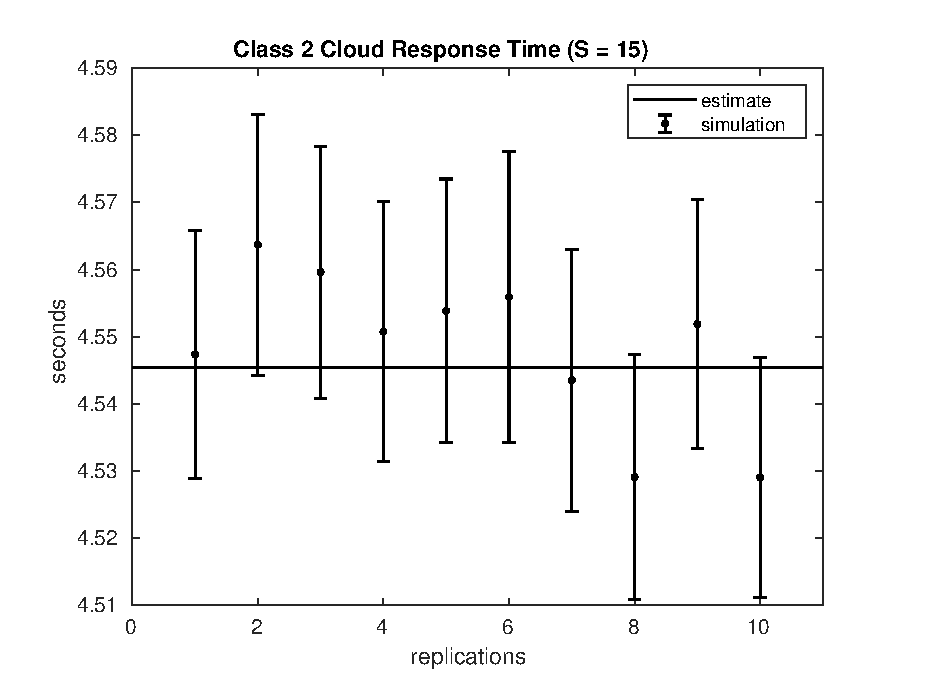
\includegraphics[width=\textwidth]{figures/simul/15_500K_s2cloud}
\caption{$S = 15$}
\label{15_s2cloud}
\end{subfigure}
%
\begin{subfigure}[t]{0.49\textwidth}
\includegraphics[width=\textwidth]{figures/simul/10_500K_s2cloud}
\caption{$S = 10$}
\label{10_s2cloud}
\end{subfigure}
%
\begin{subfigure}[t]{0.49\textwidth}
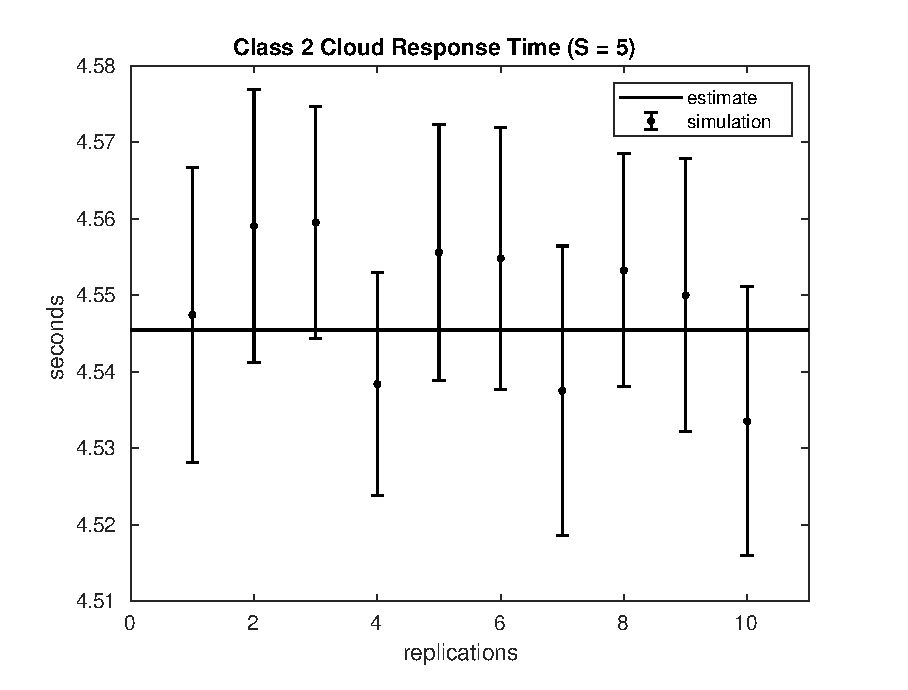
\includegraphics[width=\textwidth]{figures/simul/5_500K_s2cloud}
\caption{$S = 5$}
\label{5_s2cloud}
\end{subfigure}
%
\caption{tempo di risposta cloud classe 2}
\label{plot:s2cloud}
\end{figure}
%
%
\begin{table}[!h]
\begin{adjustbox}{width=\textwidth}
\begin{tabular}{c|r@{.}l|r@{.}l|r@{.}l|r@{.}l}
& \multicolumn{2}{|c|}{$S=20$}
& \multicolumn{2}{|c|}{$S=15$} 
& \multicolumn{2}{|c|}{$S=10$} 
& \multicolumn{2}{|c}{$S=5$} 
\\          
\hline
R1      & $4$&$5450 \pm 0.0196$  & $4$&$5474 \pm 0.0184$ & $4$&$5460 \pm 0.0188$ & $4$&$5474 \pm 0.0192$ \\
R2      & $4$&$5636 \pm 0.0219$  & $4$&$5637 \pm 0.0194$ & $4$&$5591 \pm 0.0179$ & $4$&$5590 \pm 0.0179$ \\
R3      & $4$&$5644 \pm 0.0216$  & $4$&$5596 \pm 0.0188$ & $4$&$5597 \pm 0.0165$ & $4$&$5595 \pm 0.0152$ \\
R4      & $4$&$5335 \pm 0.0185$  & $4$&$5507 \pm 0.0193$ & $4$&$5376 \pm 0.0154$ & $4$&$5384 \pm 0.0146$ \\
R5      & $4$&$5436 \pm 0.0187$  & $4$&$5538 \pm 0.0196$ & $4$&$5560 \pm 0.0148$ & $4$&$5556 \pm 0.0168$ \\
R6      & $4$&$5520 \pm 0.0221$  & $4$&$5559 \pm 0.0216$ & $4$&$5512 \pm 0.0183$ & $4$&$5548 \pm 0.0171$ \\
R7      & $4$&$5626 \pm 0.0226$  & $4$&$5435 \pm 0.0195$ & $4$&$5353 \pm 0.0186$ & $4$&$5375 \pm 0.0189$ \\
R8      & $4$&$5537 \pm 0.0195$  & $4$&$5291 \pm 0.0182$ & $4$&$5308 \pm 0.0156$ & $4$&$5533 \pm 0.0152$ \\
R9      & $4$&$5409 \pm 0.0209$  & $4$&$5519 \pm 0.0185$ & $4$&$5480 \pm 0.0157$ & $4$&$5500 \pm 0.0178$ \\
R10     & $4$&$5371 \pm 0.0197$  & $4$&$5291 \pm 0.0179$ & $4$&$5319 \pm 0.0151$ & $4$&$5335 \pm 0.0176$ \\
EST     & $4$&$5455$             & $4$&$5455$            & $4$&$5455$            & $4$&$5455$            \\
\epsmx  & $0$&$0406 \ (0.9\%)$   & $0$&$0376 \ (0.8\%)$  & $0$&$0316 \ (0.7\%)$  & $0$&$0314 \ (0.7\%)$    
\end{tabular}
\end{adjustbox}
\caption{tempo di risposta cloud classe 2}
\label{tab:s2cloud}
\end{table}

%%%%%%%%%%%%%%%%%%%%%%%%%%%%%%%%%%%%%%%%%%%%%%%%%%%%%%%%%%%%%%%%%%%%%%%%%%%%%%%%%
\subsection{Tempo di Risposta Cloud}
Il tempo di risposta del cloud è completamente dominato dai job di classe 2,
infatti, come mostrano la figura~\ref{plot:scloud} e la
tabella~\ref{tab:scloud}, i risultati sono pressoché identici alla precedente
metrica.
\begin{figure}[!h]
\centering
%
\begin{subfigure}[t]{0.49\textwidth}
\includegraphics[width=\textwidth]{figures/simul/20_500K_scloud}
\caption{$S = 20$}
\label{20_scloud}
\end{subfigure}
%
\begin{subfigure}[t]{0.49\textwidth}
\includegraphics[width=\textwidth]{figures/simul/15_500K_scloud}
\caption{$S = 15$}
\label{15_scloud}
\end{subfigure}
%
\begin{subfigure}[t]{0.49\textwidth}
\includegraphics[width=\textwidth]{figures/simul/10_500K_scloud}
\caption{$S = 10$}
\label{10_scloud}
\end{subfigure}
%
\begin{subfigure}[t]{0.49\textwidth}
\includegraphics[width=\textwidth]{figures/simul/5_500K_scloud}
\caption{$S = 5$}
\label{5_scloud}
\end{subfigure}
%
\caption{tempo di risposta cloud}
\label{plot:scloud}
\end{figure}
%
%
\begin{table}[!h]
\begin{adjustbox}{width=\textwidth}
\begin{tabular}{c|r@{.}l|r@{.}l|r@{.}l|r@{.}l}
& \multicolumn{2}{|c|}{$S=20$}
& \multicolumn{2}{|c|}{$S=15$} 
& \multicolumn{2}{|c|}{$S=10$} 
& \multicolumn{2}{|c}{$S=5$} 
\\          
\hline
R1      & $4$&$5450 \pm 0.0195$ & $4$&$5471 \pm 0.0182$ & $4$&$5455 \pm 0.0187$ & $4$&$5471 \pm 0.0192$ \\
R2      & $4$&$5633 \pm 0.0220$ & $4$&$5629 \pm 0.0195$ & $4$&$5583 \pm 0.0181$ & $4$&$5580 \pm 0.0178$ \\
R3      & $4$&$5639 \pm 0.0211$ & $4$&$5589 \pm 0.0189$ & $4$&$5591 \pm 0.0164$ & $4$&$5588 \pm 0.0147$ \\
R4      & $4$&$5329 \pm 0.0188$ & $4$&$5497 \pm 0.0194$ & $4$&$5370 \pm 0.0157$ & $4$&$5376 \pm 0.0146$ \\
R5      & $4$&$5424 \pm 0.0185$ & $4$&$5532 \pm 0.0200$ & $4$&$5553 \pm 0.0146$ & $4$&$5548 \pm 0.0170$ \\
R6      & $4$&$5510 \pm 0.0217$ & $4$&$5555 \pm 0.0214$ & $4$&$5506 \pm 0.0183$ & $4$&$5542 \pm 0.0168$ \\
R7      & $4$&$5624 \pm 0.0226$ & $4$&$5424 \pm 0.0193$ & $4$&$5351 \pm 0.0186$ & $4$&$5373 \pm 0.0189$ \\
R8      & $4$&$5532 \pm 0.0195$ & $4$&$5286 \pm 0.0181$ & $4$&$5301 \pm 0.0158$ & $4$&$5523 \pm 0.0151$ \\
R9      & $4$&$5409 \pm 0.0204$ & $4$&$5512 \pm 0.0183$ & $4$&$5478 \pm 0.0159$ & $4$&$5496 \pm 0.0175$ \\
R10     & $4$&$5374 \pm 0.0197$ & $4$&$5287 \pm 0.0179$ & $4$&$5315 \pm 0.0151$ & $4$&$5330 \pm 0.0174$ \\
EST     & $4$&$5451$            & $4$&$5452$            & $4$&$5453$            & $4$&$5453$            \\
\epsmx  & $0$&$0402 \ (0.9\%)$  & $0$&$0372 \ (0.8\%)$  & $0$&$0312 \ (0.7\%)$  & $0$&$0305 \ (0.7\%)$    
\end{tabular}
\end{adjustbox}
\caption{tempo di risposta cloud}
\label{tab:scloud}
\end{table}

%%%%%%%%%%%%%%%%%%%%%%%%%%%%%%%%%%%%%%%%%%%%%%%%%%%%%%%%%%%%%%%%%%%%%%%%%%%%%%%%
\subsection{Tempo di Risposta Job Interrotti}
La figura~\ref{plot:sintr} e la tabella~\ref{tab:sintr}, confermano che il tempo
di risposta dei job interrotti ha un andamento analogo al tempo di risposta
medio dei job di classe 2 processati con successo nel cloudlet, infatti si nota
che tale tempo è direttamente proporzionale al parametro di soglia, quindi
inversamente proporzionale alla probabilità di interruzione.

Effettuando un confronto con i tempi di risposta del cloudlet, ci si rende conto
di quanto costi l'interruzione di un job ed è quindi lecito aspettarsi che
queste interruzioni incidano in maniera significativa sul tempo di risposta dei
job di classe 2 del sistema.

Anche l'errore massimo che si è commesso con la stima della statistiche, sembra
crescere con $S$, infatti per $S=5$ si ha un errore massimo dell'$1.1\%$ che
cresce fino ad arrivare al $2.5\%$ nel caso in cui $S=20$. 
\begin{figure}[!h]
\centering
%
\begin{subfigure}[t]{0.49\textwidth}
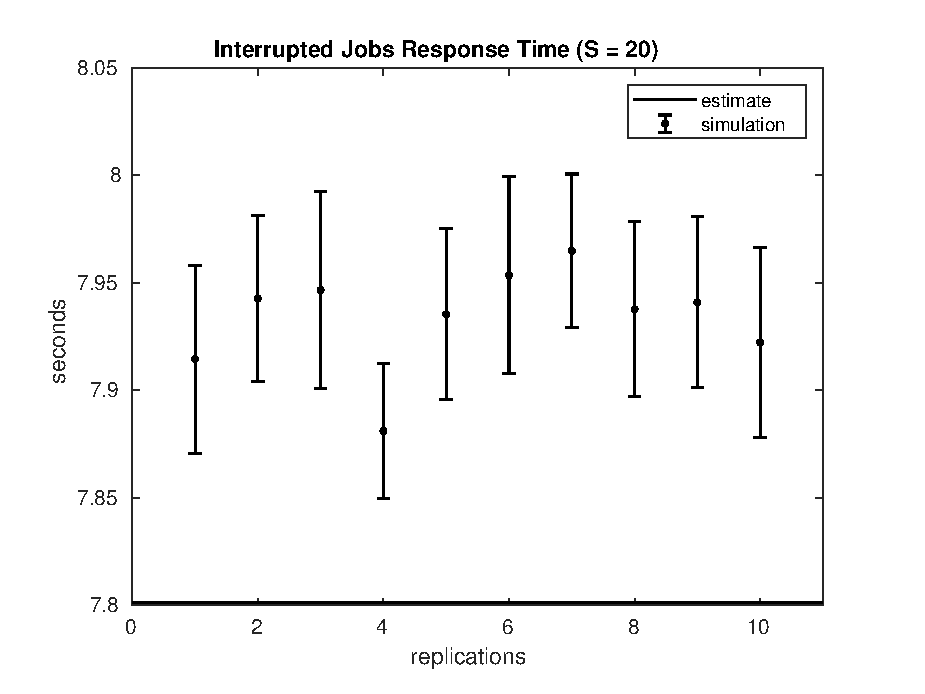
\includegraphics[width=\textwidth]{figures/simul/20_500K_sintr}
\caption{$S = 20$}
\label{20_sintr}
\end{subfigure}
%
\begin{subfigure}[t]{0.49\textwidth}
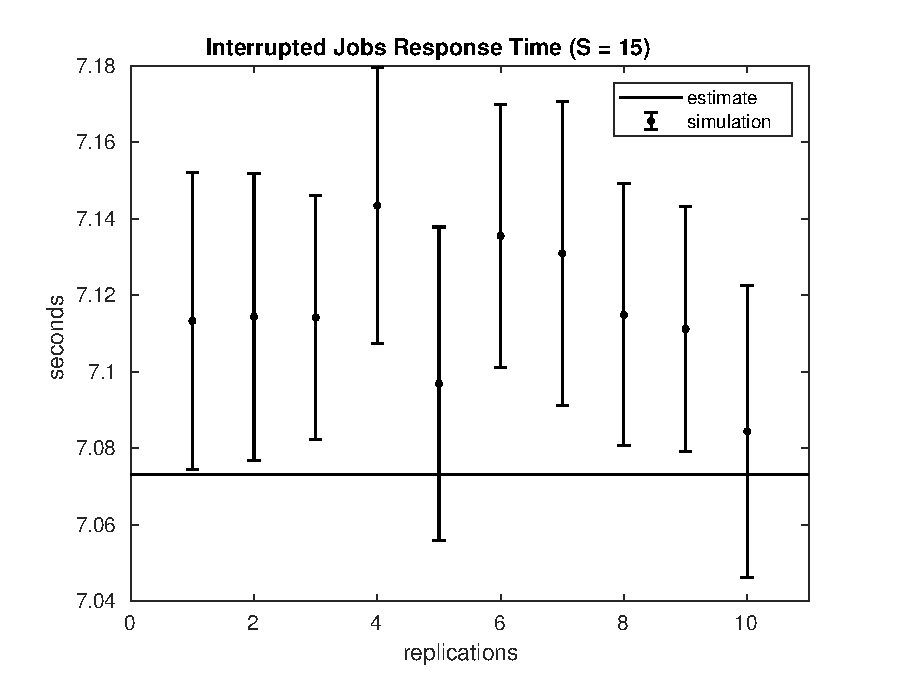
\includegraphics[width=\textwidth]{figures/simul/15_500K_sintr}
\caption{$S = 15$}
\label{15_sintr}
\end{subfigure}
%
\begin{subfigure}[t]{0.49\textwidth}
\includegraphics[width=\textwidth]{figures/simul/10_500K_sintr}
\caption{$S = 10$}
\label{10_sintr}
\end{subfigure}
%
\begin{subfigure}[t]{0.49\textwidth}
\includegraphics[width=\textwidth]{figures/simul/5_500K_sintr}
\caption{$S = 5$}
\label{5_sintr}
\end{subfigure}
%
\caption{tempo di risposta job interrotti}
\label{plot:sintr}
\end{figure}
%
%
\begin{table}[!h]
\begin{adjustbox}{width=\textwidth}
\begin{tabular}{c|r@{.}l|r@{.}l|r@{.}l|r@{.}l}
& \multicolumn{2}{|c|}{$S=20$}
& \multicolumn{2}{|c|}{$S=15$} 
& \multicolumn{2}{|c|}{$S=10$} 
& \multicolumn{2}{|c}{$S=5$} 
\\          
\hline
R1      & $7$&$9146 \pm 0.0437$  & $7$&$1133 \pm 0.0388$ & $6$&$2006 \pm 0.0381$ & $5$&$7813 \pm 0.1190$ \\
R2      & $7$&$9427 \pm 0.0387$  & $7$&$1144 \pm 0.0374$ & $6$&$2496 \pm 0.0401$ & $5$&$7846 \pm 0.1207$ \\
R3      & $7$&$9467 \pm 0.0458$  & $7$&$1142 \pm 0.0319$ & $6$&$2580 \pm 0.0342$ & $5$&$7998 \pm 0.1230$ \\
R4      & $7$&$8812 \pm 0.0312$  & $7$&$1434 \pm 0.0361$ & $6$&$2358 \pm 0.0377$ & $5$&$7744 \pm 0.1065$ \\
R5      & $7$&$9354 \pm 0.0398$  & $7$&$0969 \pm 0.0409$ & $6$&$2184 \pm 0.0373$ & $5$&$8362 \pm 0.1194$ \\
R6      & $7$&$9536 \pm 0.0457$  & $7$&$1355 \pm 0.0343$ & $6$&$2206 \pm 0.0383$ & $5$&$7372 \pm 0.1102$ \\
R7      & $7$&$9649 \pm 0.0358$  & $7$&$1309 \pm 0.0398$ & $6$&$2275 \pm 0.0441$ & $5$&$7496 \pm 0.1381$ \\
R8      & $7$&$9377 \pm 0.0407$  & $7$&$1149 \pm 0.0343$ & $6$&$1910 \pm 0.0386$ & $5$&$7802 \pm 0.1045$ \\
R9      & $7$&$9410 \pm 0.0397$  & $7$&$1112 \pm 0.0319$ & $6$&$2276 \pm 0.0365$ & $5$&$7562 \pm 0.1116$ \\
R10     & $7$&$9223 \pm 0.0443$  & $7$&$0844 \pm 0.0381$ & $6$&$2215 \pm 0.0372$ & $5$&$7570 \pm 0.1319$ \\
EST     & $7$&$8016$             & $7$&$0733$            & $6$&$3310$            & $5$&$9087$            \\
\epsmx  & $0$&$1991 \ (2.5\%)$   & $0$&$1062 \ (1.5\%)$  & $0$&$1015 \ (1.6\%)$  & $0$&$0614 \ (1.1\%)$    
\end{tabular}
\end{adjustbox}
\caption{tempo di risposta job interrotti}
\label{tab:sintr}
\end{table}

%%%%%%%%%%%%%%%%%%%%%%%%%%%%%%%%%%%%%%%%%%%%%%%%%%%%%%%%%%%%%%%%%%%%%%%%%%%%%%%%
\subsection{Tempo di Risposta Sistema Classe 1}
Il tempo di risposta globale dei job di classe 1 è completamente dominato dal
tempo di risposta dei job processati nel cloudlet, essendo molto minore il
numero di quelli eseguiti nel cloud. Infatti la figura~\ref{plot:s1} e la
tabella~\ref{tab:s1} mostrano delle statistiche pressoché identiche a quelle
relative al tempo di risposta dei job di classe 1 eseguiti nel coudlet, con un
errore massimo inferiore all'$1\%$.
\begin{figure}[!h]
\centering
%
\begin{subfigure}[t]{0.49\textwidth}
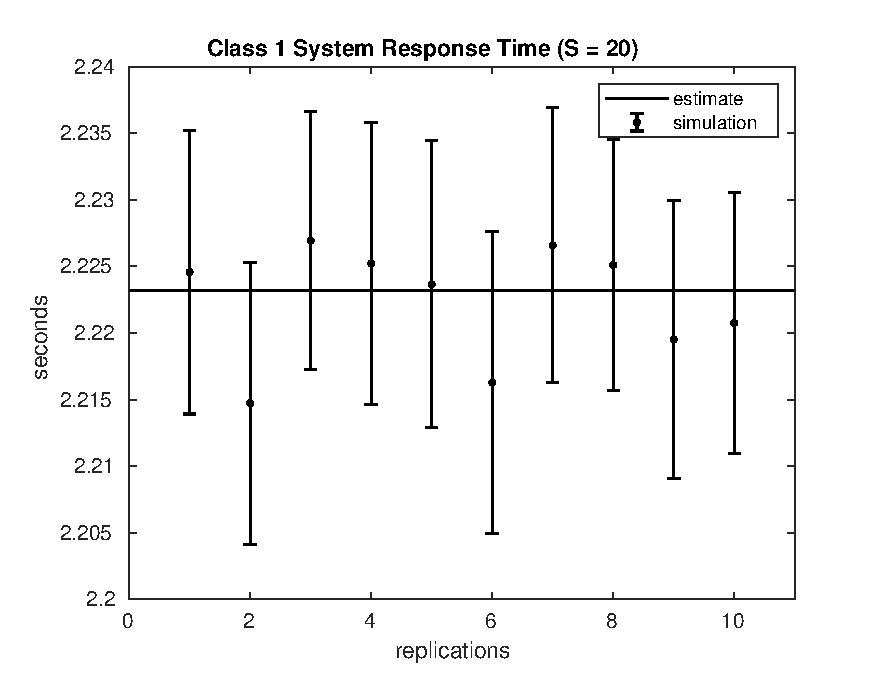
\includegraphics[width=\textwidth]{figures/simul/20_500K_s1}
\caption{$S = 20$}
\label{20_s1}
\end{subfigure}
%
\begin{subfigure}[t]{0.49\textwidth}
\includegraphics[width=\textwidth]{figures/simul/15_500K_s1}
\caption{$S = 15$}
\label{15_s1}
\end{subfigure}
%
\begin{subfigure}[t]{0.49\textwidth}
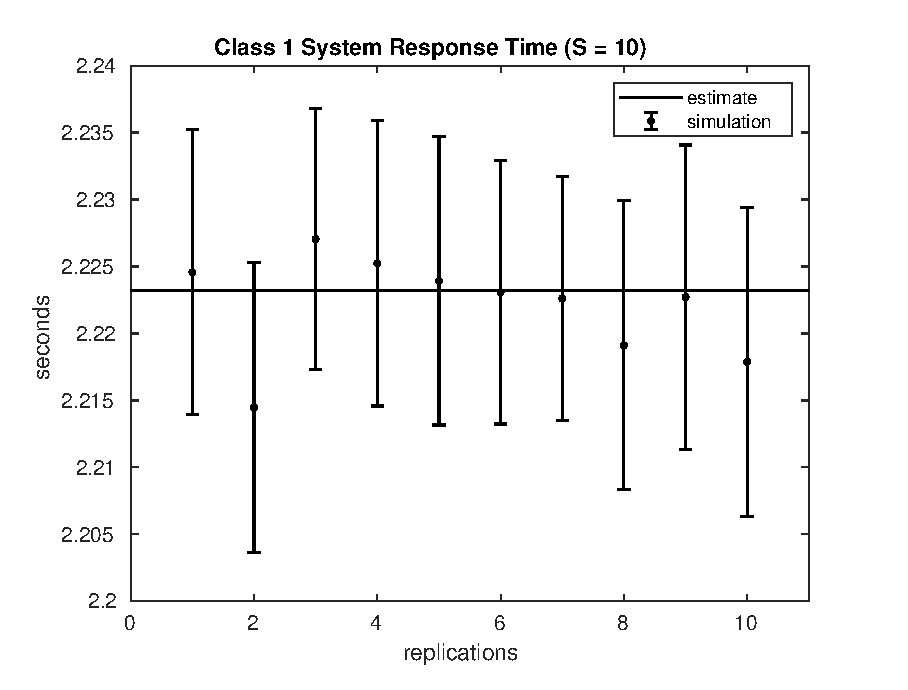
\includegraphics[width=\textwidth]{figures/simul/10_500K_s1}
\caption{$S = 10$}
\label{10_s1}
\end{subfigure}
%
\begin{subfigure}[t]{0.49\textwidth}
\includegraphics[width=\textwidth]{figures/simul/5_500K_s1}
\caption{$S = 5$}
\label{5_s1}
\end{subfigure}
%
\caption{tempo di risposta sistema classe 1}
\label{plot:s1}
\end{figure}
%
%
\begin{table}[!h]
\begin{adjustbox}{width=\textwidth}
\begin{tabular}{c|r@{.}l|r@{.}l|r@{.}l|r@{.}l}
& \multicolumn{2}{|c|}{$S=20$}
& \multicolumn{2}{|c|}{$S=15$} 
& \multicolumn{2}{|c|}{$S=10$} 
& \multicolumn{2}{|c}{$S=5$} 
\\          
\hline
R1      & $2$&$2246 \pm 0.0107$ & $2$&$2244 \pm 0.0105$ & $2$&$2246 \pm 0.0107$ & $2$&$2245 \pm 0.0106$ \\
R2      & $2$&$2147 \pm 0.0106$ & $2$&$2145 \pm 0.0110$ & $2$&$2145 \pm 0.0108$ & $2$&$2144 \pm 0.0106$ \\
R3      & $2$&$2269 \pm 0.0097$ & $2$&$2268 \pm 0.0098$ & $2$&$2270 \pm 0.0098$ & $2$&$2270 \pm 0.0099$ \\
R4      & $2$&$2252 \pm 0.0106$ & $2$&$2181 \pm 0.0103$ & $2$&$2252 \pm 0.0106$ & $2$&$2256 \pm 0.0114$ \\
R5      & $2$&$2237 \pm 0.0108$ & $2$&$2310 \pm 0.0100$ & $2$&$2239 \pm 0.0108$ & $2$&$2236 \pm 0.0101$ \\
R6      & $2$&$2163 \pm 0.0113$ & $2$&$2228 \pm 0.0107$ & $2$&$2231 \pm 0.0098$ & $2$&$2229 \pm 0.0104$ \\
R7      & $2$&$2266 \pm 0.0103$ & $2$&$2181 \pm 0.0106$ & $2$&$2226 \pm 0.0091$ & $2$&$2227 \pm 0.0095$ \\
R8      & $2$&$2251 \pm 0.0094$ & $2$&$2180 \pm 0.0102$ & $2$&$2191 \pm 0.0108$ & $2$&$2254 \pm 0.0092$ \\
R9      & $2$&$2195 \pm 0.0104$ & $2$&$2220 \pm 0.0104$ & $2$&$2227 \pm 0.0114$ & $2$&$2223 \pm 0.0107$ \\
R10     & $2$&$2208 \pm 0.0098$ & $2$&$2179 \pm 0.0120$ & $2$&$2179 \pm 0.0115$ & $2$&$2183 \pm 0.0107$ \\
EST     & $2$&$2232$            & $2$&$2232$            & $2$&$2232$            & $2$&$2232$            \\
\epsmx  & $0$&$0137 \ (0.6\%)$  & $0$&$0178 \ (0.8\%)$  & $0$&$0136 \ (0.6\%)$  & $0$&$0138 \ (0.6\%)$    
\end{tabular}
\end{adjustbox}
\caption{tempo di risposta sistema classe 1}
\label{tab:s1}
\end{table}

%%%%%%%%%%%%%%%%%%%%%%%%%%%%%%%%%%%%%%%%%%%%%%%%%%%%%%%%%%%%%%%%%%%%%%%%%%%%%%%%%
\subsection{Tempo di Risposta Sistema Classe 2}
La figura~\ref{plot:s2} e la tabella~\ref{tab:s2} mostrano che, nei casi in cui
$S=10,15,20$, i risultati delle simulazioni che risultano essere leggermente
superiori alle stime del modello analitico. Questo può essere dovuto
al peso che esercitano i job interrotti nel calcolo, infatti si ritrova la
stessa sottostima per quanto riguarda le percentuali di job interrotti
mostrate all'inizio, ma con un errore massimo minore (al più del $3.5\%$).
Inoltre nel caso in cui $S=5$, si ha una stima precisa con un errore massimo
dello $0.7\%$, perché vi sono un bassissimo numero di interruzioni.

Può essere interessante notare che si ottiene il minor tempo di risposta nello
scenario per cui $S=20$, nel quale si sperimenta il massimo tempo di risposta
dei job interrotti e una percentuale di interruzioni più alta del caso in cui si
sperimenta un tempo di risposta più basso per i job interrotti($S=10$). È
evidente quindi che acquista un peso significativo anche il tempo di esecuzione
nel cloud per quei job che ci finiscono direttamente, infatti nel caso in cui
$S=5$, nonostante soltanto circa il $2\%$ dei job viene interrotto, si registra
comunque un tempo paragonabile ai casi in cui ci sono maggiori interruzioni,
questo perché la maggior parte dei job di classe 2 viene direttamente inoltrata
al cloud.
\begin{figure}[!h]
\centering
%
\begin{subfigure}[t]{0.49\textwidth}
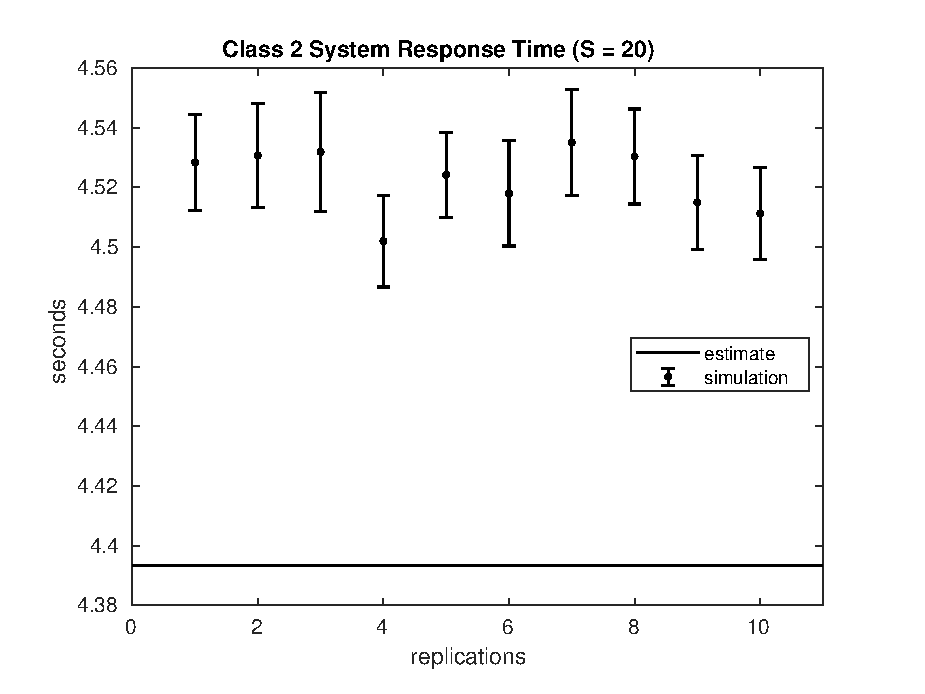
\includegraphics[width=\textwidth]{figures/simul/20_500K_s2}
\caption{$S = 20$}
\label{20_s2}
\end{subfigure}
%
\begin{subfigure}[t]{0.49\textwidth}
\includegraphics[width=\textwidth]{figures/simul/15_500K_s2}
\caption{$S = 15$}
\label{15_s2}
\end{subfigure}
%
\begin{subfigure}[t]{0.49\textwidth}
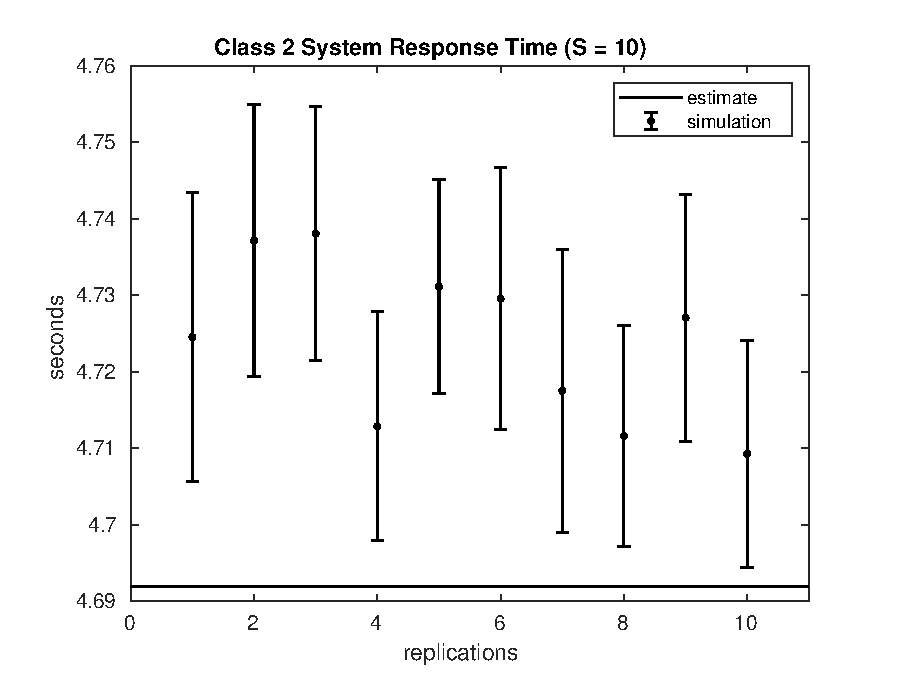
\includegraphics[width=\textwidth]{figures/simul/10_500K_s2}
\caption{$S = 10$}
\label{10_s2}
\end{subfigure}
%
\begin{subfigure}[t]{0.49\textwidth}
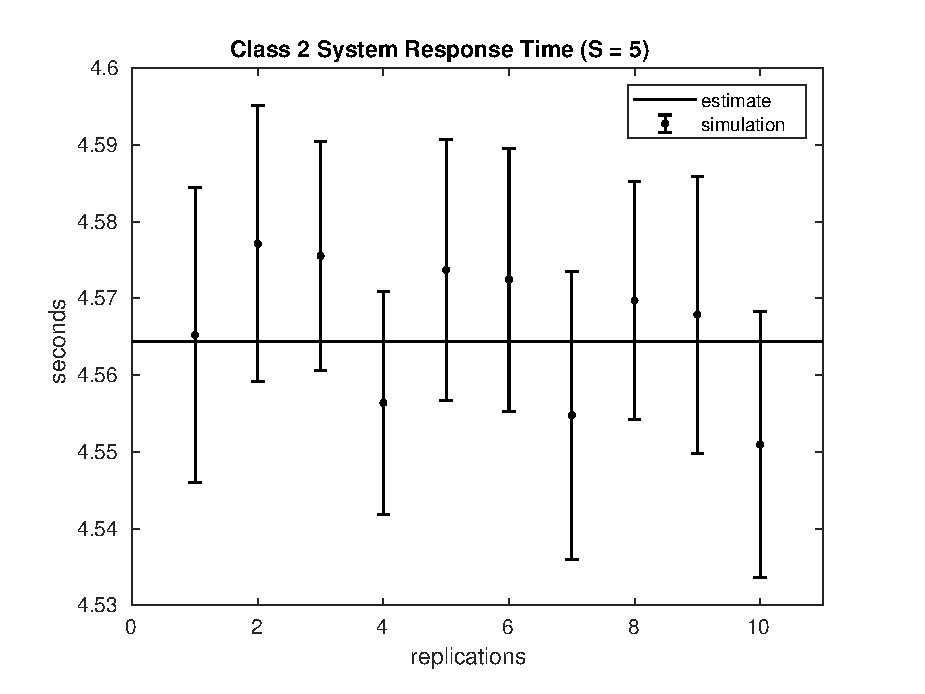
\includegraphics[width=\textwidth]{figures/simul/5_500K_s2}
\caption{$S = 5$}
\label{5_s2}
\end{subfigure}
%
\caption{tempo di risposta sistema classe 2}
\label{plot:s2}
\end{figure}
%
%
\begin{table}[!h]
\begin{adjustbox}{width=\textwidth}
\begin{tabular}{c|r@{.}l|r@{.}l|r@{.}l|r@{.}l}
& \multicolumn{2}{|c|}{$S=20$}
& \multicolumn{2}{|c|}{$S=15$} 
& \multicolumn{2}{|c|}{$S=10$} 
& \multicolumn{2}{|c}{$S=5$} 
\\          
\hline
R1      & $4$&$5284 \pm 0.0160$ & $4$&$7433 \pm 0.0154$ & $4$&$7245 \pm 0.0188$ & $4$&$5652 \pm 0.0192$ \\
R2      & $4$&$5307 \pm 0.0174$ & $4$&$7473 \pm 0.0170$ & $4$&$7371 \pm 0.0178$ & $4$&$5771 \pm 0.0180$ \\
R3      & $4$&$5319 \pm 0.0199$ & $4$&$7458 \pm 0.0185$ & $4$&$7381 \pm 0.0166$ & $4$&$5755 \pm 0.0149$ \\
R4      & $4$&$5020 \pm 0.0154$ & $4$&$7448 \pm 0.0173$ & $4$&$7129 \pm 0.0150$ & $4$&$5564 \pm 0.0145$ \\
R5      & $4$&$5242 \pm 0.0142$ & $4$&$7526 \pm 0.0181$ & $4$&$7311 \pm 0.0139$ & $4$&$5737 \pm 0.0170$ \\
R6      & $4$&$5180 \pm 0.0176$ & $4$&$7456 \pm 0.0208$ & $4$&$7295 \pm 0.0171$ & $4$&$5724 \pm 0.0171$ \\
R7      & $4$&$5351 \pm 0.0177$ & $4$&$7340 \pm 0.0164$ & $4$&$7175 \pm 0.0185$ & $4$&$5548 \pm 0.0187$ \\
R8      & $4$&$5303 \pm 0.0159$ & $4$&$7222 \pm 0.0151$ & $4$&$7116 \pm 0.0144$ & $4$&$5697 \pm 0.0155$ \\
R9      & $4$&$5150 \pm 0.0157$ & $4$&$7396 \pm 0.0168$ & $4$&$7271 \pm 0.0161$ & $4$&$5679 \pm 0.0180$ \\
R10     & $4$&$5113 \pm 0.0155$ & $4$&$7181 \pm 0.0170$ & $4$&$7093 \pm 0.0148$ & $4$&$5510 \pm 0.0173$ \\
EST     & $4$&$3935$            & $4$&$6165$            & $4$&$6920$            & $4$&$5644$            \\
\epsmx  & $0$&$1593 \ (3.5\%)$  & $0$&$1542 \ (3.2\%)$  & $0$&$0629 \ (1.3\%)$  & $0$&$0307 \ (0.7\%)$    
\end{tabular}
\end{adjustbox}
\caption{tempo di risposta sistema classe 2}
\label{tab:s2}
\end{table}

%%%%%%%%%%%%%%%%%%%%%%%%%%%%%%%%%%%%%%%%%%%%%%%%%%%%%%%%%%%%%%%%%%%%%%%%%%%%%%%%
\subsection{Tempo di Risposta Sistema}
Con l'aggiunta dei job di classe 1 nel calcolo del tempo di risposta globale del
sistema, la situazione non cambia, infatti, come mostrato in 
figura~\ref{plot:s} e tabella~\ref{tab:s}, si ottiene il minor tempo di risposta
nel caso in cui $S=20$, e anche in questo caso è evidente l'influenza della
percentuale di interruzione che induce alla sottostima, anche se con un errore
massimo più contenuto (al più del $2.7\%$), più precisa invece la stima
del caso $S=5$ (\epsmx$=0.5\%$).

In conclusione si è ottenuto che per un valore di $S=20$ si ottiene il
tempo di risposta minimo, pari a circa $3.61$ secondi, perché, con un alto
valore di soglia, si minimizzano gli inoltri diretti al cloud e si ha un numero
di interruzioni contenuto (non più del $24\%$ dei job di classe 2).
Nel caso in cui $S=15$ l'elevata percentuale di job interrotti ha influito
nell'ottenere un tempo di risposta maggiore rispetto agli altri casi, mentre per
un valore di soglia pari a $10$, nonostante il ridotto tempo di risposta dei job
interrotti e la bassa percentuale di interruzioni, si è ottenuto un tempo
maggiore dei casi $S=5,20$ per via dell'influenza dei job di classe 2 eseguiti
nel cloud

Per un valore di soglia $S=5$ si sperimenta un
elevato numero di inoltri diretti al server remoto ma al tempo stesso una
quantità minima di job interrotti, pertanto il tempo di risposta non è molto
lontano dal valore minimo che assume nel caso in cui $S=20$.

\begin{figure}[!h]
\centering
%
\begin{subfigure}[t]{0.49\textwidth}
\includegraphics[width=\textwidth]{figures/simul/20_500K_s}
\caption{$S = 20$}
\label{20_s}
\end{subfigure}
%
\begin{subfigure}[t]{0.49\textwidth}
\includegraphics[width=\textwidth]{figures/simul/15_500K_s}
\caption{$S = 15$}
\label{15_s}
\end{subfigure}
%
\begin{subfigure}[t]{0.49\textwidth}
\includegraphics[width=\textwidth]{figures/simul/10_500K_s}
\caption{$S = 10$}
\label{10_s}
\end{subfigure}
%
\begin{subfigure}[t]{0.49\textwidth}
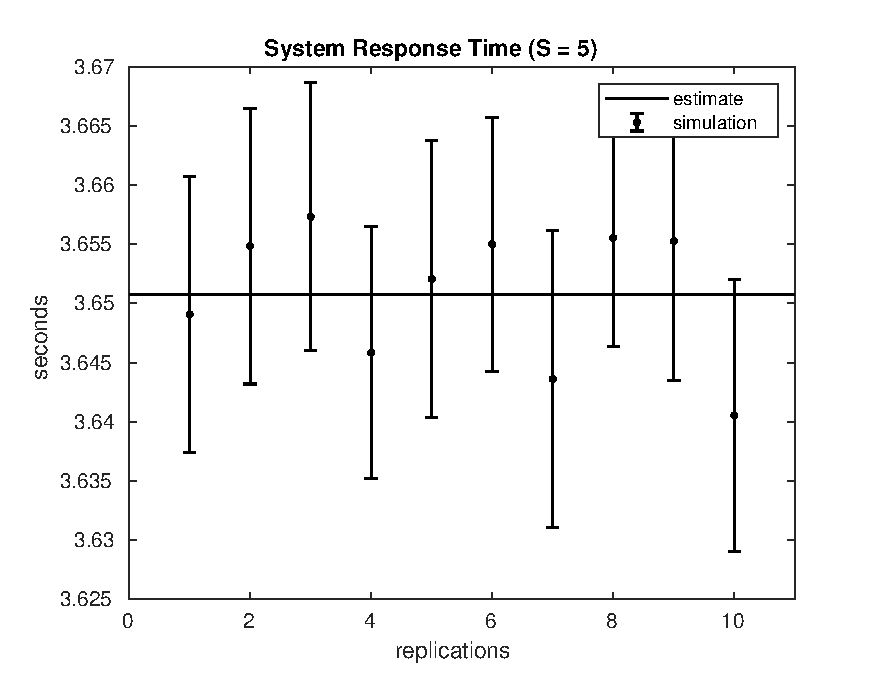
\includegraphics[width=\textwidth]{figures/simul/5_500K_s}
\caption{$S = 5$}
\label{5_s}
\end{subfigure}
%
\caption{tempo di risposta sistema}
\label{plot:s}
\end{figure}
%
%
\begin{table}[!h]
\begin{adjustbox}{width=\textwidth}
\begin{tabular}{c|r@{.}l|r@{.}l|r@{.}l|r@{.}l}
& \multicolumn{2}{|c|}{$S=20$}
& \multicolumn{2}{|c|}{$S=15$} 
& \multicolumn{2}{|c|}{$S=10$} 
& \multicolumn{2}{|c}{$S=5$} 
\\          
\hline
R1      & $3$&$6266 \pm 0.0096$ & $3$&$7575 \pm 0.0109$ & $3$&$7460 \pm 0.0129$ & $3$&$6491 \pm 0.0117$ \\
R2      & $3$&$6269 \pm 0.0121$ & $3$&$7588 \pm 0.0110$ & $3$&$7527 \pm 0.0124$ & $3$&$6548 \pm 0.0117$ \\
R3      & $3$&$6307 \pm 0.0133$ & $3$&$7611 \pm 0.0122$ & $3$&$7564 \pm 0.0114$ & $3$&$6573 \pm 0.0113$ \\
R4      & $3$&$6124 \pm 0.0110$ & $3$&$7579 \pm 0.0110$ & $3$&$7412 \pm 0.0105$ & $3$&$6458 \pm 0.0106$ \\
R5      & $3$&$6218 \pm 0.0097$ & $3$&$7675 \pm 0.0126$ & $3$&$7478 \pm 0.0103$ & $3$&$6521 \pm 0.0117$ \\
R6      & $3$&$6197 \pm 0.0125$ & $3$&$7606 \pm 0.0124$ & $3$&$7509 \pm 0.0115$ & $3$&$6550 \pm 0.0107$ \\
R7      & $3$&$6344 \pm 0.0119$ & $3$&$7539 \pm 0.0119$ & $3$&$7427 \pm 0.0120$ & $3$&$6436 \pm 0.0126$ \\
R8      & $3$&$6318 \pm 0.0103$ & $3$&$7459 \pm 0.0095$ & $3$&$7398 \pm 0.0098$ & $3$&$6555 \pm 0.0092$ \\
R9      & $3$&$6193 \pm 0.0109$ & $3$&$7603 \pm 0.0119$ & $3$&$7530 \pm 0.0114$ & $3$&$6553 \pm 0.0117$ \\
R10     & $3$&$6152 \pm 0.0100$ & $3$&$7426 \pm 0.0102$ & $3$&$7372 \pm 0.0103$ & $3$&$6406 \pm 0.0115$ \\
EST     & $3$&$5465$            & $3$&$6825$            & $3$&$7286$            & $3$&$6508$            \\
\epsmx  & $0$&$0999 \ (2.7\%)$  & $0$&$0976 \ (2.6\%)$  & $0$&$0392 \ (1.0\%)$  & $0$&$0179 \ (0.5\%)$    
\end{tabular}
\end{adjustbox}
\caption{tempo di risposta sistema}
\label{tab:s}
\end{table}

%%%%%%%%%%%%%%%%%%%%%%%%%%%%%%%%%%%%%%%%%%%%%%%%%%%%%%%%%%%%%%%%%%%%%%%%%%%%%%%%
%%%%%%%%%%%%%%%%%%%%%%%%%%%%%%%%%%%%%%%%%%%%%%%%%%%%%%%%%%%%%%%%%%%%%%%%%%%%%%%%
\subsection{Throughput Cloudlet Classe 1}
La figura~\ref{plot:x1clet} e la tabella~\ref{tab:x1clet} mostrano che il
throughput del cloudlet relativo ai job di classe 1 è pressoché costante al
variare del parametro $S$, ciò implica che l'evento in cui un job di classe 1
non viene accettato nel cloudlet avviente con probabilità remota in ogni caso.

La stima della statistica è affidabile con un errore massimo inferiore
all'$1\%$.  
\begin{figure}[!h]
\centering
%
\begin{subfigure}[t]{0.49\textwidth}
\includegraphics[width=\textwidth]{figures/simul/20_500K_x1clet}
\caption{$S = 20$}
\label{20_x1clet}
\end{subfigure}
%
\begin{subfigure}[t]{0.49\textwidth}
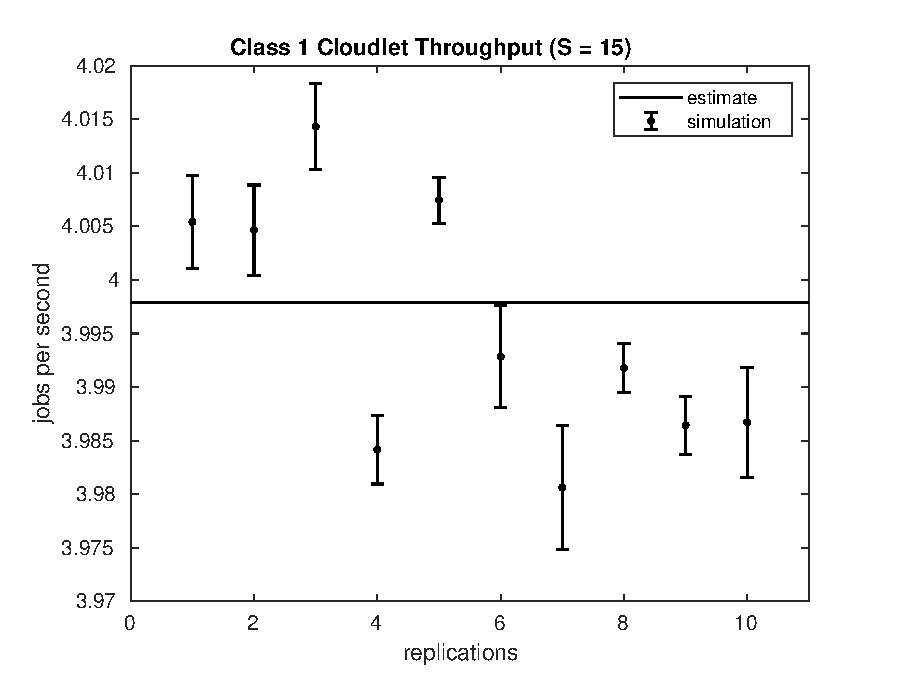
\includegraphics[width=\textwidth]{figures/simul/15_500K_x1clet}
\caption{$S = 15$}
\label{15_x1clet}
\end{subfigure}
%
\begin{subfigure}[t]{0.49\textwidth}
\includegraphics[width=\textwidth]{figures/simul/10_500K_x1clet}
\caption{$S = 10$}
\label{10_x1clet}
\end{subfigure}
%
\begin{subfigure}[t]{0.49\textwidth}
\includegraphics[width=\textwidth]{figures/simul/5_500K_x1clet}
\caption{$S = 5$}
\label{5_x1clet}
\end{subfigure}
%
\caption{throughput cloudlet classe 1}
\label{plot:x1clet}
\end{figure}
%
%
\begin{table}[!h]
\begin{adjustbox}{width=\textwidth}
\begin{tabular}{c|r@{.}l|r@{.}l|r@{.}l|r@{.}l}
& \multicolumn{2}{|c|}{$S=20$}
& \multicolumn{2}{|c|}{$S=15$}
& \multicolumn{2}{|c|}{$S=10$}
& \multicolumn{2}{|c}{$S=5$}
\\          
\hline
R1      & $4$&$0054 \pm 0.0043$ & $4$&$0054 \pm 0.0043$ & $4$&$0054 \pm 0.0043$ & $4$&$0054 \pm 0.0043$ \\
R2      & $4$&$0021 \pm 0.0048$ & $4$&$0046 \pm 0.0042$ & $4$&$0040 \pm 0.0042$ & $4$&$0037 \pm 0.0042$ \\
R3      & $4$&$0171 \pm 0.0020$ & $4$&$0143 \pm 0.0040$ & $4$&$0152 \pm 0.0033$ & $4$&$0162 \pm 0.0023$ \\
R4      & $3$&$9768 \pm 0.0043$ & $3$&$9842 \pm 0.0032$ & $3$&$9783 \pm 0.0036$ & $3$&$9741 \pm 0.0064$ \\
R5      & $4$&$0247 \pm 0.0027$ & $4$&$0074 \pm 0.0022$ & $4$&$0239 \pm 0.0028$ & $4$&$0236 \pm 0.0029$ \\
R6      & $4$&$0015 \pm 0.0022$ & $3$&$9928 \pm 0.0048$ & $3$&$9924 \pm 0.0064$ & $3$&$9907 \pm 0.0070$ \\
R7      & $4$&$0223 \pm 0.0072$ & $3$&$9806 \pm 0.0058$ & $4$&$0059 \pm 0.0083$ & $4$&$0079 \pm 0.0065$ \\
R8      & $3$&$9935 \pm 0.0108$ & $3$&$9918 \pm 0.0023$ & $3$&$9943 \pm 0.0038$ & $4$&$0059 \pm 0.0036$ \\
R9      & $3$&$9824 \pm 0.0032$ & $3$&$9864 \pm 0.0027$ & $3$&$9836 \pm 0.0032$ & $3$&$9807 \pm 0.0059$ \\
R10     & $4$&$0005 \pm 0.0033$ & $3$&$9867 \pm 0.0051$ & $3$&$9895 \pm 0.0043$ & $3$&$9874 \pm 0.0047$ \\
EST     & $3$&$9978$            & $3$&$9978$            & $3$&$9978$            & $3$&$9978$            \\
\epsmx  & $0$&$0317 \ (0.8\%)$  & $0$&$0205 \ (0.5\%)$  & $0$&$0288 \ (0.7\%)$  & $0$&$0286 \ (0.7\%)$    
\end{tabular}
\end{adjustbox}
\caption{throughput cloudlet classe 1}
\label{tab:x1clet}
\end{table}

%%%%%%%%%%%%%%%%%%%%%%%%%%%%%%%%%%%%%%%%%%%%%%%%%%%%%%%%%%%%%%%%%%%%%%%%%%%%%%%%
\subsection{Throughput Cloudlet Classe 2}
La figura~\ref{plot:x2clet} e la tabella~\ref{tab:x2clet} mostrano che il
throughput del cloudlet relativo ai job di classe 2 aumenta al crescere del
parametro $S$, di conseguenza risulta che diminuisce al crescere della
probabilità di interruzione che, poiché è sottostimata, viene prodotta un stima
maggiore dei risultati delle simulazioni.

Quindi anche questa metrica risente dell'errore di approssimazione della
percentuale di job di classe 2 interrotti, in particolare viene commesso un
errore (anch'esso proporzionale ad $S$) pari ad al più il $36\%$ nel caso in cui
$S=5$, che non è di certo trascurabile.

\begin{figure}[!h]
\centering
%
\begin{subfigure}[t]{0.49\textwidth}
\includegraphics[width=\textwidth]{figures/simul/20_500K_x2clet}
\caption{$S = 20$}
\label{20_x2clet}
\end{subfigure}
%
\begin{subfigure}[t]{0.49\textwidth}
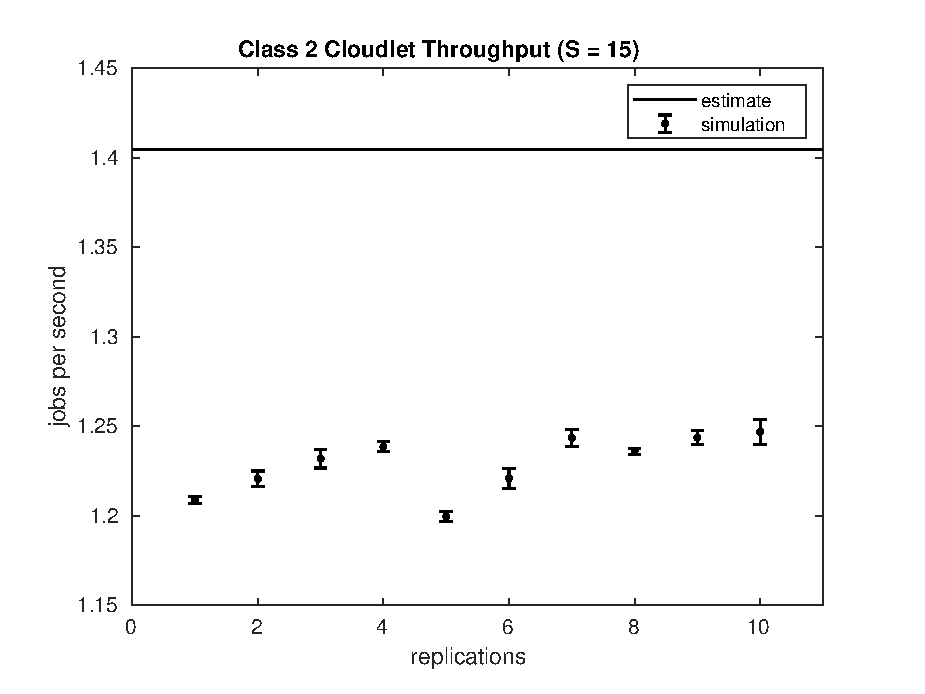
\includegraphics[width=\textwidth]{figures/simul/15_500K_x2clet}
\caption{$S = 15$}
\label{15_x2clet}
\end{subfigure}
%
\begin{subfigure}[t]{0.49\textwidth}
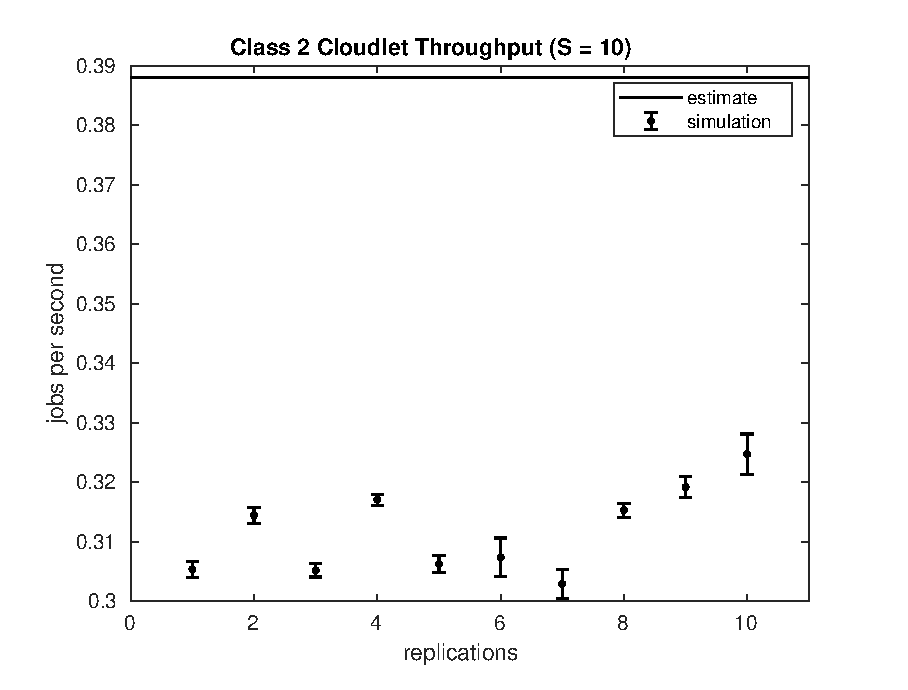
\includegraphics[width=\textwidth]{figures/simul/10_500K_x2clet}
\caption{$S = 10$}
\label{10_x2clet}
\end{subfigure}
%
\begin{subfigure}[t]{0.49\textwidth}
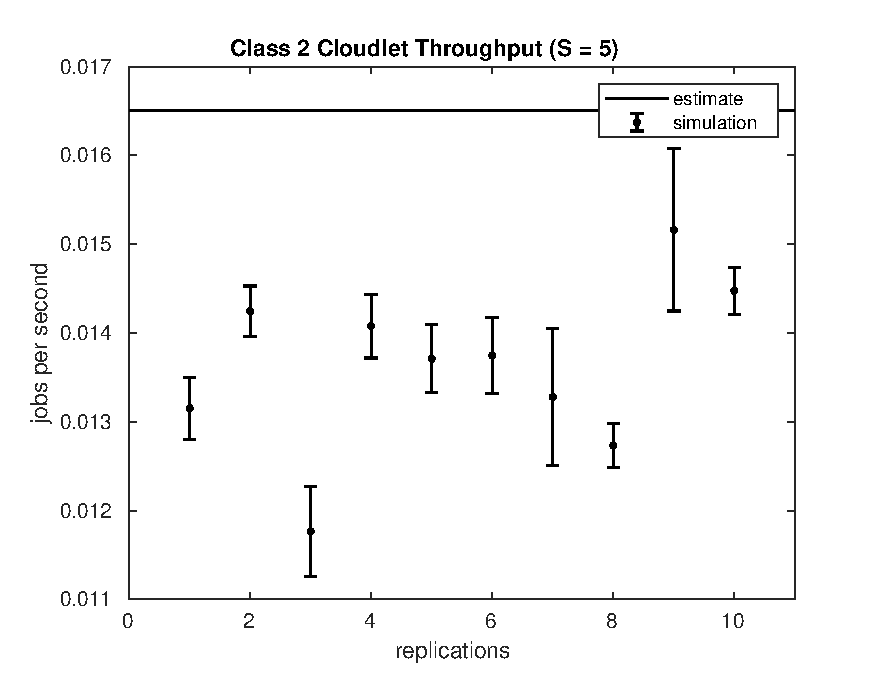
\includegraphics[width=\textwidth]{figures/simul/5_500K_x2clet}
\caption{$S = 5$}
\label{5_x2clet}
\end{subfigure}
%
\caption{throughput cloudlet classe 2}
\label{plot:x2clet}
\end{figure}
%
%
\begin{table}[!h]
\begin{adjustbox}{width=\textwidth}
\begin{tabular}{c|r@{.}l|r@{.}l|r@{.}l|r@{.}l}
& \multicolumn{2}{|c|}{$S=20$}
& \multicolumn{2}{|c|}{$S=15$}
& \multicolumn{2}{|c|}{$S=10$}
& \multicolumn{2}{|c}{$S=5$}
\\          
\hline
R1      & $2$&$4201 \pm 0.0027$ & $1$&$2090 \pm 0.0019$ & $0$&$3054 \pm 0.0013$ & $0$&$0132 \pm 0.0003$ \\
R2      & $2$&$4234 \pm 0.0058$ & $1$&$2207 \pm 0.0043$ & $0$&$3145 \pm 0.0013$ & $0$&$0142 \pm 0.0003$ \\
R3      & $2$&$4338 \pm 0.0064$ & $1$&$2320 \pm 0.0053$ & $0$&$3052 \pm 0.0011$ & $0$&$0118 \pm 0.0005$ \\
R4      & $2$&$4438 \pm 0.0019$ & $1$&$2387 \pm 0.0030$ & $0$&$3171 \pm 0.0009$ & $0$&$0141 \pm 0.0004$ \\
R5      & $2$&$3972 \pm 0.0066$ & $1$&$1996 \pm 0.0026$ & $0$&$3063 \pm 0.0014$ & $0$&$0137 \pm 0.0004$ \\
R6      & $2$&$4397 \pm 0.0048$ & $1$&$2209 \pm 0.0056$ & $0$&$3074 \pm 0.0033$ & $0$&$0137 \pm 0.0004$ \\
R7      & $2$&$4164 \pm 0.0044$ & $1$&$2436 \pm 0.0047$ & $0$&$3029 \pm 0.0025$ & $0$&$0133 \pm 0.0008$ \\
R8      & $2$&$4257 \pm 0.0084$ & $1$&$2360 \pm 0.0017$ & $0$&$3153 \pm 0.0012$ & $0$&$0127 \pm 0.0003$ \\
R9      & $2$&$4452 \pm 0.0044$ & $1$&$2436 \pm 0.0038$ & $0$&$3192 \pm 0.0018$ & $0$&$0152 \pm 0.0009$ \\
R10     & $2$&$4267 \pm 0.0035$ & $1$&$2469 \pm 0.0070$ & $0$&$3248 \pm 0.0034$ & $0$&$0145 \pm 0.0003$ \\
EST     & $2$&$5943$            & $1$&$4046$            & $0$&$3880$            & $0$&$0165$            \\
\epsmx  & $0$&$1905 \ (7.9\%)$  & $0$&$2024 \ (16.9\%)$ & $0$&$0826 \ (27.3\%)$ & $0$&$0042 \ (36.0\%)$   
\end{tabular}
\end{adjustbox}
\caption{throughput cloudlet classe 2}
\label{tab:x2clet}
\end{table}

%%%%%%%%%%%%%%%%%%%%%%%%%%%%%%%%%%%%%%%%%%%%%%%%%%%%%%%%%%%%%%%%%%%%%%%%%%%%%%%%
\subsection{Throughput Cloudlet}
La figura~\ref{plot:xclet} e la tabella~\ref{tab:xclet} mostrano che l'errore
di approssimazione dovuto alla percentuale di job interrotti viene attenuato.
Tale attenuazione risulta tanto più maggiore quanto lo è la probabilità di
interruzione, poiché ogni interruzione implica un completamento in più di classe
1, che andrà ad influire sul calcolo del throughput.

La stima della statistica è affidabile con un errore massimo che va dal $2\%$ al
$4\%$ nei casi in cui $S=10,15,20$, altrimenti nel caso in cui $S=5$ l'errore
massimo è inferiore all'$1\%$.
\begin{figure}[!h]
\centering
%
\begin{subfigure}[t]{0.49\textwidth}
\includegraphics[width=\textwidth]{figures/simul/20_500K_xclet}
\caption{$S = 20$}
\label{20_xclet}
\end{subfigure}
%
\begin{subfigure}[t]{0.49\textwidth}
\includegraphics[width=\textwidth]{figures/simul/15_500K_xclet}
\caption{$S = 15$}
\label{15_xclet}
\end{subfigure}
%
\begin{subfigure}[t]{0.49\textwidth}
\includegraphics[width=\textwidth]{figures/simul/10_500K_xclet}
\caption{$S = 10$}
\label{10_xclet}
\end{subfigure}
%
\begin{subfigure}[t]{0.49\textwidth}
\includegraphics[width=\textwidth]{figures/simul/5_500K_xclet}
\caption{$S = 5$}
\label{5_xclet}
\end{subfigure}
%
\caption{throughput cloudlet}
\label{plot:xclet}
\end{figure}
%
%
\begin{table}[!h]
\begin{adjustbox}{width=\textwidth}
\begin{tabular}{c|r@{.}l|r@{.}l|r@{.}l|r@{.}l}
& \multicolumn{2}{|c|}{$S=20$}
& \multicolumn{2}{|c|}{$S=15$}
& \multicolumn{2}{|c|}{$S=10$}
& \multicolumn{2}{|c}{$S=5$}
\\          
\hline
R1      & $6$&$4255 \pm 0.0042$ & $5$&$2144 \pm 0.0047$ & $4$&$3108 \pm 0.0047$ & $4$&$0185 \pm 0.0041$ \\
R2      & $6$&$4255 \pm 0.0030$ & $5$&$2254 \pm 0.0028$ & $4$&$3185 \pm 0.0030$ & $4$&$0179 \pm 0.0040$ \\
R3      & $6$&$4510 \pm 0.0057$ & $5$&$2463 \pm 0.0037$ & $4$&$3204 \pm 0.0030$ & $4$&$0280 \pm 0.0026$ \\
R4      & $6$&$4207 \pm 0.0036$ & $5$&$2228 \pm 0.0013$ & $4$&$2954 \pm 0.0033$ & $3$&$9881 \pm 0.0062$ \\
R5      & $6$&$4219 \pm 0.0057$ & $5$&$2071 \pm 0.0028$ & $4$&$3302 \pm 0.0032$ & $4$&$0373 \pm 0.0032$ \\
R6      & $6$&$4412 \pm 0.0043$ & $5$&$2138 \pm 0.0023$ & $4$&$2997 \pm 0.0043$ & $4$&$0044 \pm 0.0066$ \\
R7      & $6$&$4387 \pm 0.0041$ & $5$&$2242 \pm 0.0023$ & $4$&$3089 \pm 0.0064$ & $4$&$0211 \pm 0.0058$ \\
R8      & $6$&$4193 \pm 0.0033$ & $5$&$2277 \pm 0.0019$ & $4$&$3096 \pm 0.0041$ & $4$&$0186 \pm 0.0035$ \\
R9      & $6$&$4276 \pm 0.0050$ & $5$&$2300 \pm 0.0050$ & $4$&$3028 \pm 0.0041$ & $3$&$9958 \pm 0.0051$ \\
R10     & $6$&$4272 \pm 0.0021$ & $5$&$2336 \pm 0.0038$ & $4$&$3143 \pm 0.0022$ & $4$&$0019 \pm 0.0046$ \\
EST     & $6$&$5922$            & $5$&$4025$            & $4$&$3858$            & $4$&$0144$            \\
\epsmx  & $0$&$1696 \ (2.6\%)$  & $0$&$1926 \ (3.7\%)$  & $0$&$0872 \ (2.0\%)$  & $0$&$0261 \ (0.6\%)$    
\end{tabular}
\end{adjustbox}
\caption{throughput cloudlet}
\label{tab:xclet}
\end{table}

%%%%%%%%%%%%%%%%%%%%%%%%%%%%%%%%%%%%%%%%%%%%%%%%%%%%%%%%%%%%%%%%%%%%%%%%%%%%%%%%
\subsection{Throughput Sistema}
Le figure~\ref{plot:x1},~\ref{plot:x2} e~\ref{plot:x} e la
tabelle~\ref{tab:x1},~\ref{tab:x2} e~\ref{tab:x} mostrano i risultati relativi
al throughput del sistema sia per classe che globalmente, e viene confermata
l'ipotesi di stabilità sfruttata nel modello analitico, poiché le stime
approssimano bene i valori delle simulazioni con un errore massimo inferiore
all'$1\%$.
\begin{figure}[!h]
\centering
%
\begin{subfigure}[t]{0.49\textwidth}
\includegraphics[width=\textwidth]{figures/simul/20_500K_x1}
\caption{$S = 20$}
\label{20_x1}
\end{subfigure}
%
\begin{subfigure}[t]{0.49\textwidth}
\includegraphics[width=\textwidth]{figures/simul/15_500K_x1}
\caption{$S = 15$}
\label{15_x1}
\end{subfigure}
%
\begin{subfigure}[t]{0.49\textwidth}
\includegraphics[width=\textwidth]{figures/simul/10_500K_x1}
\caption{$S = 10$}
\label{10_x1}
\end{subfigure}
%
\begin{subfigure}[t]{0.49\textwidth}
\includegraphics[width=\textwidth]{figures/simul/5_500K_x1}
\caption{$S = 5$}
\label{5_x1}
\end{subfigure}
%
\caption{throughput sistema classe 1}
\label{plot:x1}
\end{figure}
%
%
\begin{table}[!h]
\begin{adjustbox}{width=\textwidth}
\begin{tabular}{c|r@{.}l|r@{.}l|r@{.}l|r@{.}l}
& \multicolumn{2}{|c|}{$S=20$}
& \multicolumn{2}{|c|}{$S=15$}
& \multicolumn{2}{|c|}{$S=10$}
& \multicolumn{2}{|c}{$S=5$}
\\          
\hline
R1      & $4$&$0067 \pm 0.0044$ & $4$&$0067 \pm 0.0043$ & $4$&$0067 \pm 0.0044$ & $4$&$0067 \pm 0.0044$ \\
R2      & $4$&$0056 \pm 0.0050$ & $4$&$0082 \pm 0.0044$ & $4$&$0076 \pm 0.0044$ & $4$&$0072 \pm 0.0044$ \\
R3      & $4$&$0187 \pm 0.0021$ & $4$&$0158 \pm 0.0041$ & $4$&$0167 \pm 0.0033$ & $4$&$0178 \pm 0.0024$ \\
R4      & $3$&$9789 \pm 0.0044$ & $3$&$9865 \pm 0.0032$ & $3$&$9803 \pm 0.0037$ & $3$&$9761 \pm 0.0065$ \\
R5      & $4$&$0268 \pm 0.0027$ & $4$&$0095 \pm 0.0022$ & $4$&$0260 \pm 0.0028$ & $4$&$0257 \pm 0.0029$ \\
R6      & $4$&$0035 \pm 0.0022$ & $3$&$9947 \pm 0.0048$ & $3$&$9942 \pm 0.0065$ & $3$&$9925 \pm 0.0071$ \\
R7      & $4$&$0246 \pm 0.0073$ & $3$&$9830 \pm 0.0059$ & $4$&$0084 \pm 0.0084$ & $4$&$0109 \pm 0.0059$ \\
R8      & $3$&$9964 \pm 0.0109$ & $3$&$9941 \pm 0.0023$ & $3$&$9967 \pm 0.0037$ & $4$&$0089 \pm 0.0036$ \\
R9      & $3$&$9844 \pm 0.0032$ & $3$&$9885 \pm 0.0028$ & $3$&$9852 \pm 0.0032$ & $3$&$9827 \pm 0.0059$ \\
R10     & $4$&$0034 \pm 0.0034$ & $3$&$9887 \pm 0.0051$ & $3$&$9916 \pm 0.0042$ & $3$&$9894 \pm 0.0046$ \\
EST     & $4$&$0000$            & $4$&$0000$            & $4$&$0000$            & $4$&$0000$            \\
\epsmx  & $0$&$0319 \ (0.8\%)$  & $0$&$0199 \ (0.5\%)$  & $0$&$0288 \ (0.7\%)$  & $0$&$0286 \ (0.7\%)$    
\end{tabular}
\end{adjustbox}
\caption{throughput sistema classe 1}
\label{tab:x1}
\end{table}

%%%%%%%%%%%%%%%%%%%%%%%%%%%%%%%%%%%%%%%%%%%%%%%%%%%%%%%%%%%%%%%%%%%%%%%%%%%%%%%%
\begin{figure}[!h]
\centering
%
\begin{subfigure}[t]{0.49\textwidth}
\includegraphics[width=\textwidth]{figures/simul/20_500K_x2}
\caption{$S = 20$}
\label{20_x2}
\end{subfigure}
%
\begin{subfigure}[t]{0.49\textwidth}
\includegraphics[width=\textwidth]{figures/simul/15_500K_x2}
\caption{$S = 15$}
\label{15_x2}
\end{subfigure}
%
\begin{subfigure}[t]{0.49\textwidth}
\includegraphics[width=\textwidth]{figures/simul/10_500K_x2}
\caption{$S = 10$}
\label{10_x2}
\end{subfigure}
%
\begin{subfigure}[t]{0.49\textwidth}
\includegraphics[width=\textwidth]{figures/simul/5_500K_x2}
\caption{$S = 5$}
\label{5_x2}
\end{subfigure}
%
\caption{throughput sistema classe 2}
\label{plot:x2}
\end{figure}
%
%
\begin{table}[!h]
\begin{adjustbox}{width=\textwidth}
\begin{tabular}{c|r@{.}l|r@{.}l|r@{.}l|r@{.}l}
& \multicolumn{2}{|c|}{$S=20$}
& \multicolumn{2}{|c|}{$S=15$}
& \multicolumn{2}{|c|}{$S=10$}
& \multicolumn{2}{|c}{$S=5$}
\\          
\hline
R1      & $6$&$2431 \pm 0.0101$ & $6$&$2428 \pm 0.0103$ & $6$&$2429 \pm 0.0103$ & $6$&$2430 \pm 0.0102$ \\
R2      & $6$&$2230 \pm 0.0072$ & $6$&$2229 \pm 0.0076$ & $6$&$2231 \pm 0.0074$ & $6$&$2232 \pm 0.0074$ \\
R3      & $6$&$2559 \pm 0.0083$ & $6$&$2556 \pm 0.0084$ & $6$&$2556 \pm 0.0085$ & $6$&$2557 \pm 0.0084$ \\
R4      & $6$&$2282 \pm 0.0068$ & $6$&$2366 \pm 0.0088$ & $6$&$2274 \pm 0.0076$ & $6$&$2314 \pm 0.0042$ \\
R5      & $6$&$2075 \pm 0.0044$ & $6$&$2562 \pm 0.0092$ & $6$&$2053 \pm 0.0063$ & $6$&$2051 \pm 0.0063$ \\
R6      & $6$&$2481 \pm 0.0048$ & $6$&$2355 \pm 0.0115$ & $6$&$2381 \pm 0.0109$ & $6$&$2373 \pm 0.0114$ \\
R7      & $6$&$2753 \pm 0.0061$ & $6$&$2301 \pm 0.0117$ & $6$&$2683 \pm 0.0027$ & $6$&$2725 \pm 0.0032$ \\
R8      & $6$&$2661 \pm 0.0055$ & $6$&$2477 \pm 0.0023$ & $6$&$2461 \pm 0.0029$ & $6$&$2623 \pm 0.0054$ \\
R9      & $6$&$2387 \pm 0.0061$ & $6$&$2753 \pm 0.0060$ & $6$&$2744 \pm 0.0066$ & $6$&$2755 \pm 0.0065$ \\
R10     & $6$&$2370 \pm 0.0029$ & $6$&$2272 \pm 0.0104$ & $6$&$2276 \pm 0.0105$ & $6$&$2261 \pm 0.0108$ \\
EST     & $6$&$2500$            & $6$&$2500$            & $6$&$2500$            & $6$&$2500$            \\
\epsmx  & $0$&$0381 \ (0.6\%)$  & $0$&$0313 \ (0.5\%)$  & $0$&$0384 \ (0.6\%)$  & $0$&$0386 \ (0.6\%)$    
\end{tabular}
\end{adjustbox}
\caption{throughput sistema classe 2}
\label{tab:x2}
\end{table}

%%%%%%%%%%%%%%%%%%%%%%%%%%%%%%%%%%%%%%%%%%%%%%%%%%%%%%%%%%%%%%%%%%%%%%%%%%%%%%%%
\begin{figure}[!h]
\centering
%
\begin{subfigure}[t]{0.49\textwidth}
\includegraphics[width=\textwidth]{figures/simul/20_500K_x}
\caption{$S = 20$}
\label{20_x}
\end{subfigure}
%
\begin{subfigure}[t]{0.49\textwidth}
\includegraphics[width=\textwidth]{figures/simul/15_500K_x}
\caption{$S = 15$}
\label{15_x}
\end{subfigure}
%
\begin{subfigure}[t]{0.49\textwidth}
\includegraphics[width=\textwidth]{figures/simul/10_500K_x}
\caption{$S = 10$}
\label{10_x}
\end{subfigure}
%
\begin{subfigure}[t]{0.49\textwidth}
\includegraphics[width=\textwidth]{figures/simul/5_500K_x}
\caption{$S = 5$}
\label{5_x}
\end{subfigure}
%
\caption{throughput sistema}
\label{plot:x}
\end{figure}
%
%
\begin{table}[!h]
\begin{adjustbox}{width=\textwidth}
\begin{tabular}{c|r@{.}l|r@{.}l|r@{.}l|r@{.}l}
& \multicolumn{2}{|c|}{$S=20$}
& \multicolumn{2}{|c|}{$S=15$}
& \multicolumn{2}{|c|}{$S=10$}
& \multicolumn{2}{|c}{$S=5$}
\\          
\hline
R1      & $10$&$2498 \pm 0.0138$ & $10$&$2496 \pm 0.0140$ & $10$&$2496 \pm 0.0140$ & $10$&$2497 \pm 0.0139$ \\
R2      & $10$&$2286 \pm 0.0076$ & $10$&$2311 \pm 0.0056$ & $10$&$2306 \pm 0.0060$ & $10$&$2303 \pm 0.0062$ \\
R3      & $10$&$2746 \pm 0.0088$ & $10$&$2714 \pm 0.0116$ & $10$&$2723 \pm 0.0108$ & $10$&$2734 \pm 0.0095$ \\
R4      & $10$&$2071 \pm 0.0102$ & $10$&$2231 \pm 0.0105$ & $10$&$2077 \pm 0.0096$ & $10$&$2075 \pm 0.0098$ \\
R5      & $10$&$2343 \pm 0.0042$ & $10$&$2656 \pm 0.0105$ & $10$&$2313 \pm 0.0069$ & $10$&$2308 \pm 0.0072$ \\
R6      & $10$&$2516 \pm 0.0039$ & $10$&$2302 \pm 0.0154$ & $10$&$2323 \pm 0.0168$ & $10$&$2298 \pm 0.0180$ \\
R7      & $10$&$2999 \pm 0.0086$ & $10$&$2132 \pm 0.0174$ & $10$&$2766 \pm 0.0097$ & $10$&$2834 \pm 0.0048$ \\
R8      & $10$&$2625 \pm 0.0117$ & $10$&$2418 \pm 0.0033$ & $10$&$2428 \pm 0.0037$ & $10$&$2712 \pm 0.0071$ \\
R9      & $10$&$2231 \pm 0.0085$ & $10$&$2638 \pm 0.0072$ & $10$&$2596 \pm 0.0090$ & $10$&$2582 \pm 0.0116$ \\
R10     & $10$&$2404 \pm 0.0038$ & $10$&$2160 \pm 0.0143$ & $10$&$2192 \pm 0.0121$ & $10$&$2156 \pm 0.0142$ \\
EST     & $10$&$2500$            & $10$&$2500$            & $10$&$2500$            & $10$&$2500$            \\
\epsmx  & $0$&$0584 \ (0.6\%)$   & $0$&$0330 \ (0.3\%)$   & $0$&$0363 \ (0.4\%)$   & $0$&$0382 \ (0.4\%)$     
\end{tabular}
\end{adjustbox}
\caption{throughput sistema}
\label{tab:x}
\end{table}

%%%%%%%%%%%%%%%%%%%%%%%%%%%%%%%%%%%%%%%%%%%%%%%%%%%%%%%%%%%%%%%%%%%%%%%%%%%%%%%%
\subsection{Popolazione Cloudlet Classe 1}
La figura~\ref{plot:n1clet} e la tabella~\ref{tab:n1clet} mostrano che i valori
della popolazione media per i job di classe nel cloudlet sono pressoché costanti
al variare del parametro $S$, a causa della bassa probabilità che un job di
classe 1 venga inviato al server remoto. La stima approssima bene i risultati
con un errore massimo pari all'$1\%$.
\begin{figure}[!h]
\centering
%
\begin{subfigure}[t]{0.49\textwidth}
\includegraphics[width=\textwidth]{figures/simul/20_500K_n1clet}
\caption{$S = 20$}
\label{20_n1clet}
\end{subfigure}
%
\begin{subfigure}[t]{0.49\textwidth}
\includegraphics[width=\textwidth]{figures/simul/15_500K_n1clet}
\caption{$S = 15$}
\label{15_n1clet}
\end{subfigure}
%
\begin{subfigure}[t]{0.49\textwidth}
\includegraphics[width=\textwidth]{figures/simul/10_500K_n1clet}
\caption{$S = 10$}
\label{10_n1clet}
\end{subfigure}
%
\begin{subfigure}[t]{0.49\textwidth}
\includegraphics[width=\textwidth]{figures/simul/5_500K_n1clet}
\caption{$S = 5$}
\label{5_n1clet}
\end{subfigure}
%
\caption{popolazione cloudlet classe 1}
\label{plot:n1clet}
\end{figure}
%
%
\begin{table}[!h]
\begin{adjustbox}{width=\textwidth}
\begin{tabular}{c|r@{.}l|r@{.}l|r@{.}l|r@{.}l}
& \multicolumn{2}{|c|}{$S=20$}
& \multicolumn{2}{|c|}{$S=15$}
& \multicolumn{2}{|c|}{$S=10$}
& \multicolumn{2}{|c}{$S=5$}
\\          
\hline
R1      & $8$&$9175 \pm 0.0070$ & $8$&$9175 \pm 0.0070$ & $8$&$9175 \pm 0.0070$ & $8$&$9175 \pm 0.0070$ \\
R2      & $8$&$8757 \pm 0.0154$ & $8$&$8834 \pm 0.0158$ & $8$&$8801 \pm 0.0152$ & $8$&$8783 \pm 0.0152$ \\
R3      & $8$&$9431 \pm 0.0074$ & $8$&$9370 \pm 0.0124$ & $8$&$9380 \pm 0.0115$ & $8$&$9399 \pm 0.0095$ \\
R4      & $8$&$8371 \pm 0.0222$ & $8$&$8193 \pm 0.0098$ & $8$&$8389 \pm 0.0202$ & $8$&$8367 \pm 0.0212$ \\
R5      & $8$&$9625 \pm 0.0149$ & $8$&$9151 \pm 0.0082$ & $8$&$9575 \pm 0.0109$ & $8$&$9462 \pm 0.0100$ \\
R6      & $8$&$8553 \pm 0.0072$ & $8$&$8850 \pm 0.0185$ & $8$&$8816 \pm 0.0205$ & $8$&$8722 \pm 0.0232$ \\
R7      & $8$&$9466 \pm 0.0131$ & $8$&$7982 \pm 0.0242$ & $8$&$9220 \pm 0.0190$ & $8$&$9277 \pm 0.0165$ \\
R8      & $8$&$8924 \pm 0.0302$ & $8$&$8328 \pm 0.0074$ & $8$&$8451 \pm 0.0088$ & $8$&$9244 \pm 0.0106$ \\
R9      & $8$&$8399 \pm 0.0127$ & $8$&$8353 \pm 0.0060$ & $8$&$8301 \pm 0.0065$ & $8$&$8258 \pm 0.0122$ \\
R10     & $8$&$8683 \pm 0.0112$ & $8$&$7973 \pm 0.0210$ & $8$&$8036 \pm 0.0176$ & $8$&$7986 \pm 0.0187$ \\
EST     & $8$&$8841$            & $8$&$8841$            & $8$&$8841$            & $8$&$8841$            \\
\epsmx  & $0$&$0933 \ (1.0\%)$  & $0$&$0659 \ (0.7\%)$  & $0$&$0842 \ (0.9\%)$  & $0$&$0721 \ (0.8\%)$    
\end{tabular}
\end{adjustbox}
\caption{popolazione cloudlet classe 1}
\label{tab:n1clet}
\end{table}

%%%%%%%%%%%%%%%%%%%%%%%%%%%%%%%%%%%%%%%%%%%%%%%%%%%%%%%%%%%%%%%%%%%%%%%%%%%%%%%%
\subsection{Popolazione Cloudlet Classe 2}
La figura~\ref{plot:n2clet} e la tabella~\ref{tab:n2clet} mostrano che la
popolazione media dei job di classe 2 diminuisce al decrescere del parametro
$S$, ciò è lecito poiché con l'abbassamento del valore di soglia vengono
accettati sempre meno job di classe 2.

La stima commette un'errore che invece aumenta al decrescere di $S$,
probabilmente dovuto a inprecisioni della distribuzione stazionaria, che saranno
anche la causa del valore approssimato della percentuale di interruzione.
\begin{figure}[!h]
\centering
%
\begin{subfigure}[t]{0.49\textwidth}
\includegraphics[width=\textwidth]{figures/simul/20_500K_n2clet}
\caption{$S = 20$}
\label{20_n2clet}
\end{subfigure}
%
\begin{subfigure}[t]{0.49\textwidth}
\includegraphics[width=\textwidth]{figures/simul/15_500K_n2clet}
\caption{$S = 15$}
\label{15_n2clet}
\end{subfigure}
%
\begin{subfigure}[t]{0.49\textwidth}
\includegraphics[width=\textwidth]{figures/simul/10_500K_n2clet}
\caption{$S = 10$}
\label{10_n2clet}
\end{subfigure}
%
\begin{subfigure}[t]{0.49\textwidth}
\includegraphics[width=\textwidth]{figures/simul/5_500K_n2clet}
\caption{$S = 5$}
\label{5_n2clet}
\end{subfigure}
%
\caption{popolazione cloudlet classe 2}
\label{plot:n2clet}
\end{figure}
%
%
\begin{table}[!h]
\begin{adjustbox}{width=\textwidth}
\begin{tabular}{c|r@{.}l|r@{.}l|r@{.}l|r@{.}l}
& \multicolumn{2}{|c|}{$S=20$}
& \multicolumn{2}{|c|}{$S=15$}
& \multicolumn{2}{|c|}{$S=10$}
& \multicolumn{2}{|c}{$S=5$}
\\          
\hline
R1      & $9$&$6707 \pm 0.0069$ & $5$&$2295 \pm 0.0069$ & $1$&$4243 \pm 0.0045$ & $0$&$0613 \pm 0.0011$ \\
R2      & $9$&$6856 \pm 0.0183$ & $5$&$2579 \pm 0.0164$ & $1$&$4540 \pm 0.0095$ & $0$&$0652 \pm 0.0015$ \\
R3      & $9$&$6394 \pm 0.0059$ & $5$&$2088 \pm 0.0076$ & $1$&$3996 \pm 0.0042$ & $0$&$0558 \pm 0.0007$ \\
R4      & $9$&$7394 \pm 0.0208$ & $5$&$3249 \pm 0.0077$ & $1$&$4784 \pm 0.0068$ & $0$&$0638 \pm 0.0014$ \\
R5      & $9$&$6128 \pm 0.0188$ & $5$&$2324 \pm 0.0070$ & $1$&$4243 \pm 0.0041$ & $0$&$0637 \pm 0.0008$ \\
R6      & $9$&$7140 \pm 0.0089$ & $5$&$2611 \pm 0.0164$ & $1$&$4530 \pm 0.0106$ & $0$&$0605 \pm 0.0018$ \\
R7      & $9$&$6312 \pm 0.0120$ & $5$&$3423 \pm 0.0192$ & $1$&$4291 \pm 0.0097$ & $0$&$0587 \pm 0.0014$ \\
R8      & $9$&$6854 \pm 0.0230$ & $5$&$3087 \pm 0.0054$ & $1$&$4778 \pm 0.0062$ & $0$&$0594 \pm 0.0010$ \\
R9      & $9$&$7243 \pm 0.0092$ & $5$&$3002 \pm 0.0068$ & $1$&$4780 \pm 0.0039$ & $0$&$0662 \pm 0.0018$ \\
R10     & $9$&$7099 \pm 0.0093$ & $5$&$3322 \pm 0.0171$ & $1$&$4895 \pm 0.0111$ & $0$&$0669 \pm 0.0012$ \\
EST     & $9$&$6087$            & $5$&$2024$            & $1$&$4370$            & $0$&$0611$            \\
\epsmx  & $0$&$1515 \ (1.6\%)$  & $0$&$1592 \ (3.0\%)$  & $0$&$0637 \ (4.3\%)$  & $0$&$0069 \ (10.3\%)$   
\end{tabular}
\end{adjustbox}
\caption{popolazione cloudlet classe 2}
\label{tab:n2clet}
\end{table}

%%%%%%%%%%%%%%%%%%%%%%%%%%%%%%%%%%%%%%%%%%%%%%%%%%%%%%%%%%%%%%%%%%%%%%%%%%%%%%%%
\subsection{Popolazione Cloud Classe 1}
La figura~\ref{plot:n1cloud} e la tabella~\ref{tab:n1cloud} mostrano la
popolazione media del cloudlet relativa ai job di classe 1 prossima allo 0, per
il solito motivo della remota probabilità di blocco.

Il numero di job è talmente basso, che ogni replica della simulazione può
produrre risultati molto variegati, infatti vengono prodotti intarvalli di
confidenza ampi e la stima del modello analitico può commettere un errore anche
del $65\%$.
\begin{figure}[!h]
\centering
%
\begin{subfigure}[t]{0.49\textwidth}
\includegraphics[width=\textwidth]{figures/simul/20_500K_n1cloud}
\caption{$S = 20$}
\label{20_n1cloud}
\end{subfigure}
%
\begin{subfigure}[t]{0.49\textwidth}
\includegraphics[width=\textwidth]{figures/simul/15_500K_n1cloud}
\caption{$S = 15$}
\label{15_n1cloud}
\end{subfigure}
%
\begin{subfigure}[t]{0.49\textwidth}
\includegraphics[width=\textwidth]{figures/simul/10_500K_n1cloud}
\caption{$S = 10$}
\label{10_n1cloud}
\end{subfigure}
%
\begin{subfigure}[t]{0.49\textwidth}
\includegraphics[width=\textwidth]{figures/simul/5_500K_n1cloud}
\caption{$S = 5$}
\label{5_n1cloud}
\end{subfigure}
%
\caption{popolazione cloud classe 1}
\label{plot:n1cloud}
\end{figure}
%
%
\begin{table}[!h]
\begin{adjustbox}{width=\textwidth}
\begin{tabular}{c|r@{.}l|r@{.}l|r@{.}l|r@{.}l}
& \multicolumn{2}{|c|}{$S=20$}
& \multicolumn{2}{|c|}{$S=15$}
& \multicolumn{2}{|c|}{$S=10$}
& \multicolumn{2}{|c}{$S=5$}
\\          
\hline
R1      & $0$&$0049 \pm 0.0004$ & $0$&$0049 \pm 0.0004$ & $0$&$0049 \pm 0.0004$ & $0$&$0049 \pm 0.0004$ \\
R2      & $0$&$0183 \pm 0.0024$ & $0$&$0164 \pm 0.0019$ & $0$&$0170 \pm 0.0019$ & $0$&$0143 \pm 0.0017$ \\
R3      & $0$&$0063 \pm 0.0005$ & $0$&$0052 \pm 0.0004$ & $0$&$0053 \pm 0.0004$ & $0$&$0062 \pm 0.0004$ \\
R4      & $0$&$0097 \pm 0.0005$ & $0$&$0103 \pm 0.0007$ & $0$&$0084 \pm 0.0008$ & $0$&$0079 \pm 0.0007$ \\
R5      & $0$&$0076 \pm 0.0003$ & $0$&$0063 \pm 0.0006$ & $0$&$0088 \pm 0.0006$ & $0$&$0074 \pm 0.0005$ \\
R6      & $0$&$0079 \pm 0.0004$ & $0$&$0064 \pm 0.0003$ & $0$&$0067 \pm 0.0003$ & $0$&$0061 \pm 0.0003$ \\
R7      & $0$&$0113 \pm 0.0006$ & $0$&$0070 \pm 0.0005$ & $0$&$0099 \pm 0.0005$ & $0$&$0109 \pm 0.0016$ \\
R8      & $0$&$0125 \pm 0.0007$ & $0$&$0082 \pm 0.0005$ & $0$&$0086 \pm 0.0005$ & $0$&$0124 \pm 0.0006$ \\
R9      & $0$&$0061 \pm 0.0005$ & $0$&$0062 \pm 0.0002$ & $0$&$0060 \pm 0.0005$ & $0$&$0087 \pm 0.0007$ \\
R10     & $0$&$0126 \pm 0.0006$ & $0$&$0074 \pm 0.0005$ & $0$&$0073 \pm 0.0003$ & $0$&$0078 \pm 0.0005$ \\
EST     & $0$&$0086$            & $0$&$0086$            & $0$&$0086$            & $0$&$0086$            \\
\epsmx  & $0$&$0121 \ (65.9\%)$ & $0$&$0098 \ (59.3\%)$ & $0$&$0103 \ (60.5\%)$ & $0$&$0074 \ (51.9\%)$   
\end{tabular}
\end{adjustbox}
\caption{popolazione cloud classe 1}
\label{tab:n1cloud}
\end{table}

%%%%%%%%%%%%%%%%%%%%%%%%%%%%%%%%%%%%%%%%%%%%%%%%%%%%%%%%%%%%%%%%%%%%%%%%%%%%%%%%
\subsection{Popolazione Cloud Classe 2}
La popolazione media del cloud relativa ai job di classe 2 varia in maniera
opposta alla popolazione media del cloudlet, infatti cresce all'aumentare della
probabilità di interruzione. 

La figura~\ref{plot:n2cloud} e la tabella~\ref{tab:n2cloud} mostrano i risultati
delle simulazioni a confronto con le stime del modello analitico e, anche per
quanto riguarda l'errore massimo, si ha un andamento inverso a quello relativo
al cloudlet, infatti l'errore massimo aumenta al crescere di $S$. Inoltre, nei
casi in cui $S=10,15,20$, la stima è leggermente inferiore ai risultati poiché
il tasso di arrivo al nodo è proporzionale alla percentuale di interruzione,
pertanto anche in questo caso ci si porta dietro l'errore di approssimazione.
\begin{figure}[!h]
\centering
%
\begin{subfigure}[t]{0.49\textwidth}
\includegraphics[width=\textwidth]{figures/simul/20_500K_n2cloud}
\caption{$S = 20$}
\label{20_n2cloud}
\end{subfigure}
%
\begin{subfigure}[t]{0.49\textwidth}
\includegraphics[width=\textwidth]{figures/simul/15_500K_n2cloud}
\caption{$S = 15$}
\label{15_n2cloud}
\end{subfigure}
%
\begin{subfigure}[t]{0.49\textwidth}
\includegraphics[width=\textwidth]{figures/simul/10_500K_n2cloud}
\caption{$S = 10$}
\label{10_n2cloud}
\end{subfigure}
%
\begin{subfigure}[t]{0.49\textwidth}
\includegraphics[width=\textwidth]{figures/simul/5_500K_n2cloud}
\caption{$S = 5$}
\label{5_n2cloud}
\end{subfigure}
%
\caption{popolazione cloud classe 2}
\label{plot:n2cloud}
\end{figure}
%
%
\begin{table}[!h]
\begin{adjustbox}{width=\textwidth}
\begin{tabular}{c|r@{.}l|r@{.}l|r@{.}l|r@{.}l}
& \multicolumn{2}{|c|}{$S=20$}
& \multicolumn{2}{|c|}{$S=15$}
& \multicolumn{2}{|c|}{$S=10$}
& \multicolumn{2}{|c}{$S=5$}
\\          
\hline
R1      & $17$&$3911 \pm 0.0508$ & $22$&$8912 \pm 0.0481$ & $26$&$9995 \pm 0.0462$ & $28$&$3291 \pm 0.0487$ \\
R2      & $17$&$3631 \pm 0.0287$ & $22$&$8482 \pm 0.0162$ & $26$&$9781 \pm 0.0227$ & $28$&$3499 \pm 0.0253$ \\
R3      & $17$&$4461 \pm 0.0659$ & $22$&$9171 \pm 0.0713$ & $27$&$1424 \pm 0.0596$ & $28$&$4834 \pm 0.0558$ \\
R4      & $17$&$1158 \pm 0.0384$ & $22$&$7350 \pm 0.0544$ & $26$&$7608 \pm 0.0387$ & $28$&$1584 \pm 0.0248$ \\
R5      & $17$&$2666 \pm 0.0249$ & $22$&$9743 \pm 0.0370$ & $26$&$7727 \pm 0.0602$ & $28$&$1037 \pm 0.0637$ \\
R6      & $17$&$2828 \pm 0.0251$ & $23$&$0087 \pm 0.0723$ & $27$&$1679 \pm 0.0611$ & $28$&$5090 \pm 0.0511$ \\
R7      & $17$&$6046 \pm 0.0309$ & $22$&$5677 \pm 0.0975$ & $27$&$0170 \pm 0.0386$ & $28$&$3535 \pm 0.0312$ \\
R8      & $17$&$5160 \pm 0.0511$ & $22$&$6737 \pm 0.0178$ & $26$&$8463 \pm 0.0144$ & $28$&$5050 \pm 0.0216$ \\
R9      & $17$&$2087 \pm 0.0371$ & $22$&$9575 \pm 0.0283$ & $27$&$1525 \pm 0.0322$ & $28$&$5347 \pm 0.0399$ \\
R10     & $17$&$2797 \pm 0.0190$ & $22$&$5209 \pm 0.0901$ & $26$&$6949 \pm 0.0772$ & $28$&$0868 \pm 0.0725$ \\
EST     & $16$&$6166$            & $22$&$0244$            & $26$&$6456$            & $28$&$3341$            \\
\epsmx  & $1$&$0188 \ (5.8\%)$   & $1$&$0567 \ (4.6\%)$   & $0$&$5835 \ (2.1\%)$   & $0$&$2405 \ (0.8\%)$     
\end{tabular}
\end{adjustbox}
\caption{popolazione cloud classe 2}
\label{tab:n2cloud}
\end{table}

%%%%%%%%%%%%%%%%%%%%%%%%%%%%%%%%%%%%%%%%%%%%%%%%%%%%%%%%%%%%%%%%%%%%%%%%%%%%%%%%
%%%%%%%%%%%%%%%%%%%%%%%%%%%%%%%%%%%%%%%%%%%%%%%%%%%%%%%%%%%%%%%%%%%%%%%%%%%%%%%%
